\clearpage
\section{Kramers-Kronig PAM Transceiver}

\begin{tcolorbox}	
\begin{tabular}{p{2.75cm} p{0.2cm} p{10.5cm}} 	
\textbf{Student Name}  &:& Romil Patel\\
\textbf{Starting Date} &:& August 16, 2017\\
\textbf{Goal}          &:& Develop a simplified structure (low cost) for a coherent receiver, that can be used in coherent PON, inter-data center connections, or metropolitan networks (optical path lengths < 100 km).
\end{tabular}
\end{tcolorbox}

%In recent days, homodyne detection has been discussed and investigated a lot due to the advancement in the DSP in the electrical domain. However, a major drawback of homodyne detection is the incoming signal should be separated into inphase and quadrature (I/Q) signals in the optical domain. Therefore, it demands more hardware to accommodate the requirement of the signal separation  in the optical domain. For instance, 4 balanced photodetectors with double hybrid structures and 4-channel ADCs are required.
%On the other hand, heterodyne receiver simplifies the detection scheme to some extent with the requirement of having only half of photodetectors and ADC.\\
Coherent optical transmission schemes are spectrally efficient since they allow the encoding of information in both quadrature of sinusoid signal. Coherent detection schemes constitute the solution for the medium-to-long-reach optical transmission links; however, the cost of coherent receiver becomes a major obstacle in the case of short-reach links applications like PON, inter-data-center communications and metropolitan network. In order to get rid of higher cost and to make the transceiver applicable in short-reach links, a new architecture of optical receiver has been proposed which combines the advantages of coherent transmission and cost effectiveness of direct detection. The working principle of the proposed transceiver is based on the famous Kramers-Kronig (KK) relationship. The KK transceiver scheme allows digital compensation of linear propagation impairment, and it is efficient in terms of spectral occupancy and energy consumption. 
\subsection{Concept of Kramers-Kronig receiver }
%The key concept behind the Kramers-Kronig self coherent receiver is to aquire "\textit{minimum phase single sideband signal}".
The proposed receiver scheme allows the full reconstruction of the complex-valued signal from the amplitude data. 

\subsubsection{1. What are the requirements for the KK receiver scheme?}
The Kramers-Kronig receiver based communication scheme relies on identifying a condition which ensures that \textbf{the received signal is minimum phase}, in such a case its phase can be uniquely extracted from its intensity[2].\\ In order to facilitate the extraction of phase information from the intensity of the received minimum phase signal, it is prerequisite that the transmitted signal should be \textbf{analytical signal} in which real and imaginary parts are related to each other by means of Hilbert transform of each other.

\subsubsection{2. What is minimum phase signal?}
A necessary and sufficient condition for a complex signal $A(t)$ to be minimum phase is that the curve described in a complex plane by $A(t)$ when $t\rightarrow -\infty$ to $t\rightarrow \infty$ \textbf{does not encircle the origin}.

\subsubsection{3. What is Analytical Signal?}
An analytic signal is a complex-valued signal that has no negative frequency components, and its real and imaginary parts are related to each other by the Hilbert transform (See Appendix A for what is Hilbert transform?).
\begin{equation}
s_a(t)=s(t)+i\hat{s}(t)
\label{Analytical signal}
\end{equation}
where, $s_a(t)$ is an analytical signal and $\hat{s}(t)$ is the Hilbert transform of the signal ${s}(t)$. Such analytical signal can be used to generate Single Sideband Signal (SSB) signal (See the Appendix B).

\subsubsection{4. How we can use these signals and profit from them?}
This section represents the justification that why we need to use these signals into our proposed transceiver system.\\
\textbf{Analytical Signal:}\\
Analytical signal used for generating single sidebnad (SSB) signal. In the case of a SSB signal $A_s(t)$ described as,
\begin{equation}
A_s(t)=A_{s,r}(t)+iA_{s,i}(t)
\label{5.15}
\end{equation}
the real part $A_{s,r}(t)$  and the imaginary parts $A_{s,i}(t)$ are Hilbert transform of each other as (See Appendix C)[3],
\begin{equation}
\begin{split}
A_{s,r}(t) &=-\frac{1}{\pi} p.v. \int_{-\infty}^{\infty} \frac{A_{s,i}(t')}{t-t'} dt' \\
A_{s,i}(t) &=\frac{1}{\pi} p.v. \int_{-\infty}^{\infty} \frac{A_{s,r}(t')}{t-t'} dt' \\
\end{split}
\label{E}
\end{equation}
These relations are known as Kramers-Kronig relation. We can define this Kramers-Kronig relationship into the following simplified form,
\begin{equation}
\begin{split}
A_{s}(t) &=\frac{i}{\pi} p.v. \int_{-\infty}^{\infty} \frac{A_{s}(t')}{t-t'} dt' 
\end{split}
\label{Eq:5.17}
\end{equation}\\
\textbf{Minimum Phase signal:}\\
If the trajectory of the received SSB signal $A(t)=A_{s}(t)+\bar{A}$ never encircles the origin for $t\in(-\infty,\infty)$ then its phase can be reconstructed by a logarithmaic Hilbert transform of its amplitude (See Appendix D)[3],
\begin{equation}
\phi(t) = \bar{\phi} + \dfrac{1}{2\pi} p.v. \int_{-\infty}^{\infty} \dfrac{log[|A(t')|^2]}{t-t'} dt'
\end{equation}\\
where the $A(t)=|A(t)|exp(i\phi(t))$ and $\bar{A}=|\bar{E}|exp(i\bar{\phi})$.

%The communication scheme discussed here relies on the identifying a specific condition that ensures the received signal is minimum phase. This condition facilitates the unique way to extract the phase of the received signal from its intensity. If we denote s(t) as a complex data-carrying signals whose spectrum is contained between -B/2 to B/2, and consider a single sideband signal of the form,
%\begin{equation}
%h(t)=A+s(t)exp(i\pi Bt)
%\end{equation}
%Where $A$ is a constant. Here, Nyquist stability criterion can be used to ensure that $s(t)$ is a minimum phase signal. The condition of minimum phase signal is satisfied when $|A|>|s(t)|$ by guaranteeing Nyquist stability of the received signal.
%When $h(t)$ is a minimum-phase signal, its phase $\phi(t)$ and absolute value $|h(t)|$ are uniquely related by Hilbert transform:
%\begin{equation}
%	\phi(t)=\frac{1}{\pi}  p.v. \int_{-\infty}^{\infty} dt' \frac{log[|h(t')|]}{t-t'}
%	\label{Eq:5.15}
%\end{equation}
%where \textit{p.v.} stands for \textit{principal value}. The relationship depicted in Equation \ref{Eq:5.15} can also be conveniently implemented in frequency domain as,
%\begin{equation}
%\tilde{\phi}(\omega)=i sign(\omega) \mathcal{F} \{log[|h(t)|]\}
%\label{Eq:5.16}
%\end{equation}
%where $sign(\omega)$ is the sign function which is equal to 1 when $\omega>0$, to 0 when $\omega=0$ and to -1 when $\omega<0$. Symbol $\mathcal{F}$ denotes the Fourier transform.

\subsection{KK scheme}
If we consider the complex envelope of the incoming electric field by $A_s(t)$ confined within the optical bandwidth denoted by B. The LO assumed to be a continuous wave (CW) signal whose amplitude is $A_0$ whose frequency coincides with the left edge of the information-carrying signal spectrum. Here, we assumed that $A_0$ is real-valued and positive, which is equivalent to referring all phase value to that of LO.\\
The complex envelope of the field striking upon the photo-diode can be given as,
\begin{equation}
A(t)=A_s(t)+A_0 exp(i\pi Bt)
\end{equation}
The photo current $I$ produced by the photo-diode is proportional to the field intensity $I=|A(t)|^2$, here proportionality constant considered as 1 for the sake of simplicity. If $A_0$ is large enough to ensure that the signal $A(t)exp(-i\pi Bt)=A_0+A_s(t)exp(-i\pi Bt)$ is minimum phase. The discussed hypothesis can be used to reconstruct the signal $E_s(t)$ as follows[1]:
\begin{equation}
A_s(t)=\{\sqrt{I(t)} exp[i\phi_E(t)]-A_0\} exp(i\pi Bt)
\end{equation}
\begin{equation}
\phi_A(t)=\dfrac{1}{2\pi} p.v. \int_{-\infty}^{\infty} dt' \frac{log[|I(t')|]}{t-t'}
\label{Eq:5.19}
\end{equation}
%Here, the average value of the phase returned by Equation \ref{Eq:5.19} is zero, which implies the need for an additional phase-recovery procedure. 
%\begin{figure}[h]
%	\centering
%	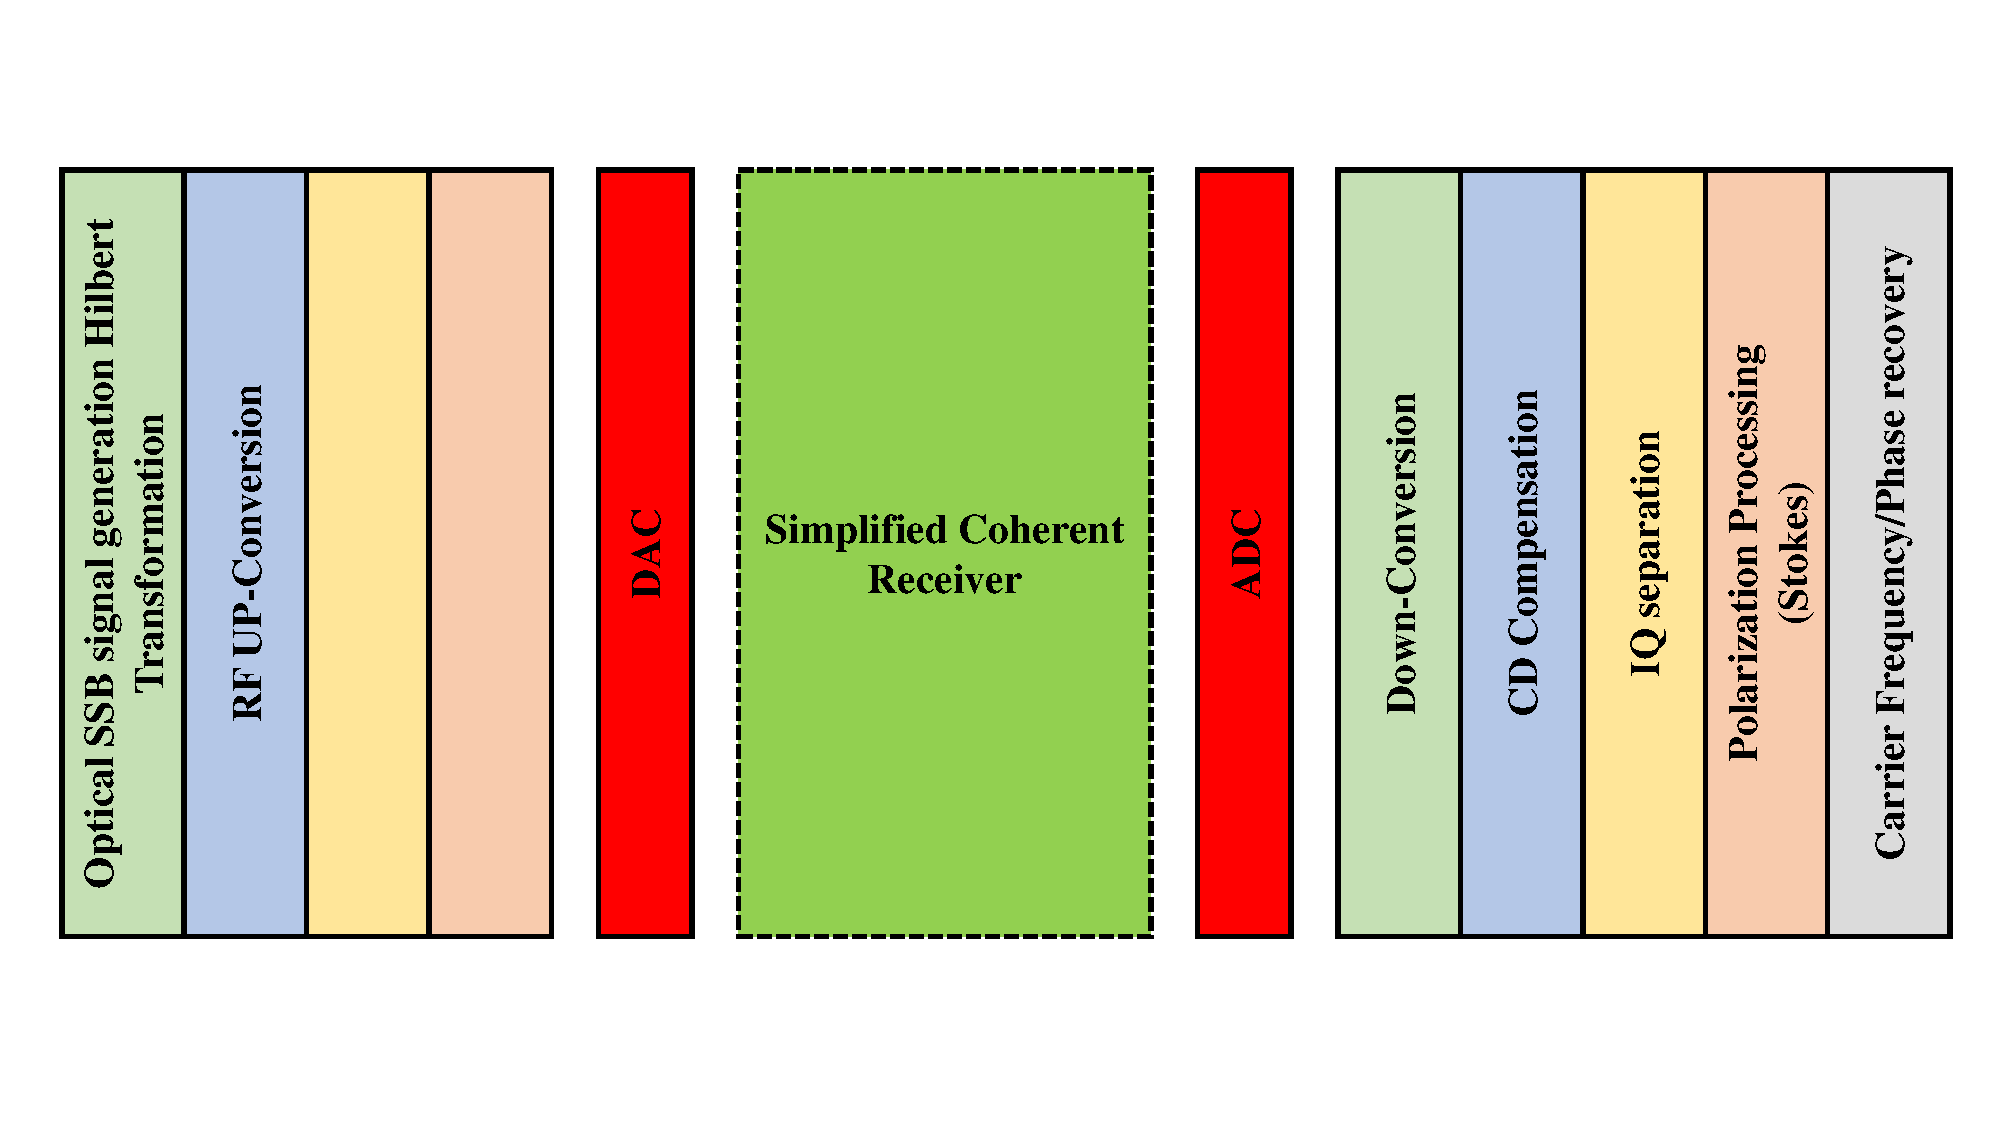
\includegraphics[width=1.0\textwidth, height=8cm]{./sdf/simplified_coherent_receiver/figures/detailed_subsystem.pdf}
%	\caption{Tx/Rx DSP main subsystem}\label{DSP_main_subsystem}
%\end{figure}

\subsection{Simulation set-up}
\subsubsection{Tx side}
At the transmitter side (Figure \ref{Simulation_setup_Tx}), random bit sequence generated and mapped it to MPAM symbol. After mapping, MPAM signal passed through the RRC filter and up-converted to form a band-limited signal $s(t)$. As per the requirement of KK receiver, it is a prerequisite that the transmitted signal needs to be an analytical signal. In the analytical signal $s_a(t)$, imaginary part $\hat{s}(t)$ is Hilbert transformed version of signal $s(t)$. Real part  $s(t)$ of the analytical signal  $s_a(t)$ applied to one quadrature of the IQ modulator and imaginary part  $\hat{s}(t)$ applied to the other quadrature. As discussed earlier, the output of the IQ modulator will generate single sideband (SSB) signal $A_s(t)$ that will be launched into the optical fiber.
\begin{figure}[h]
	\centering
	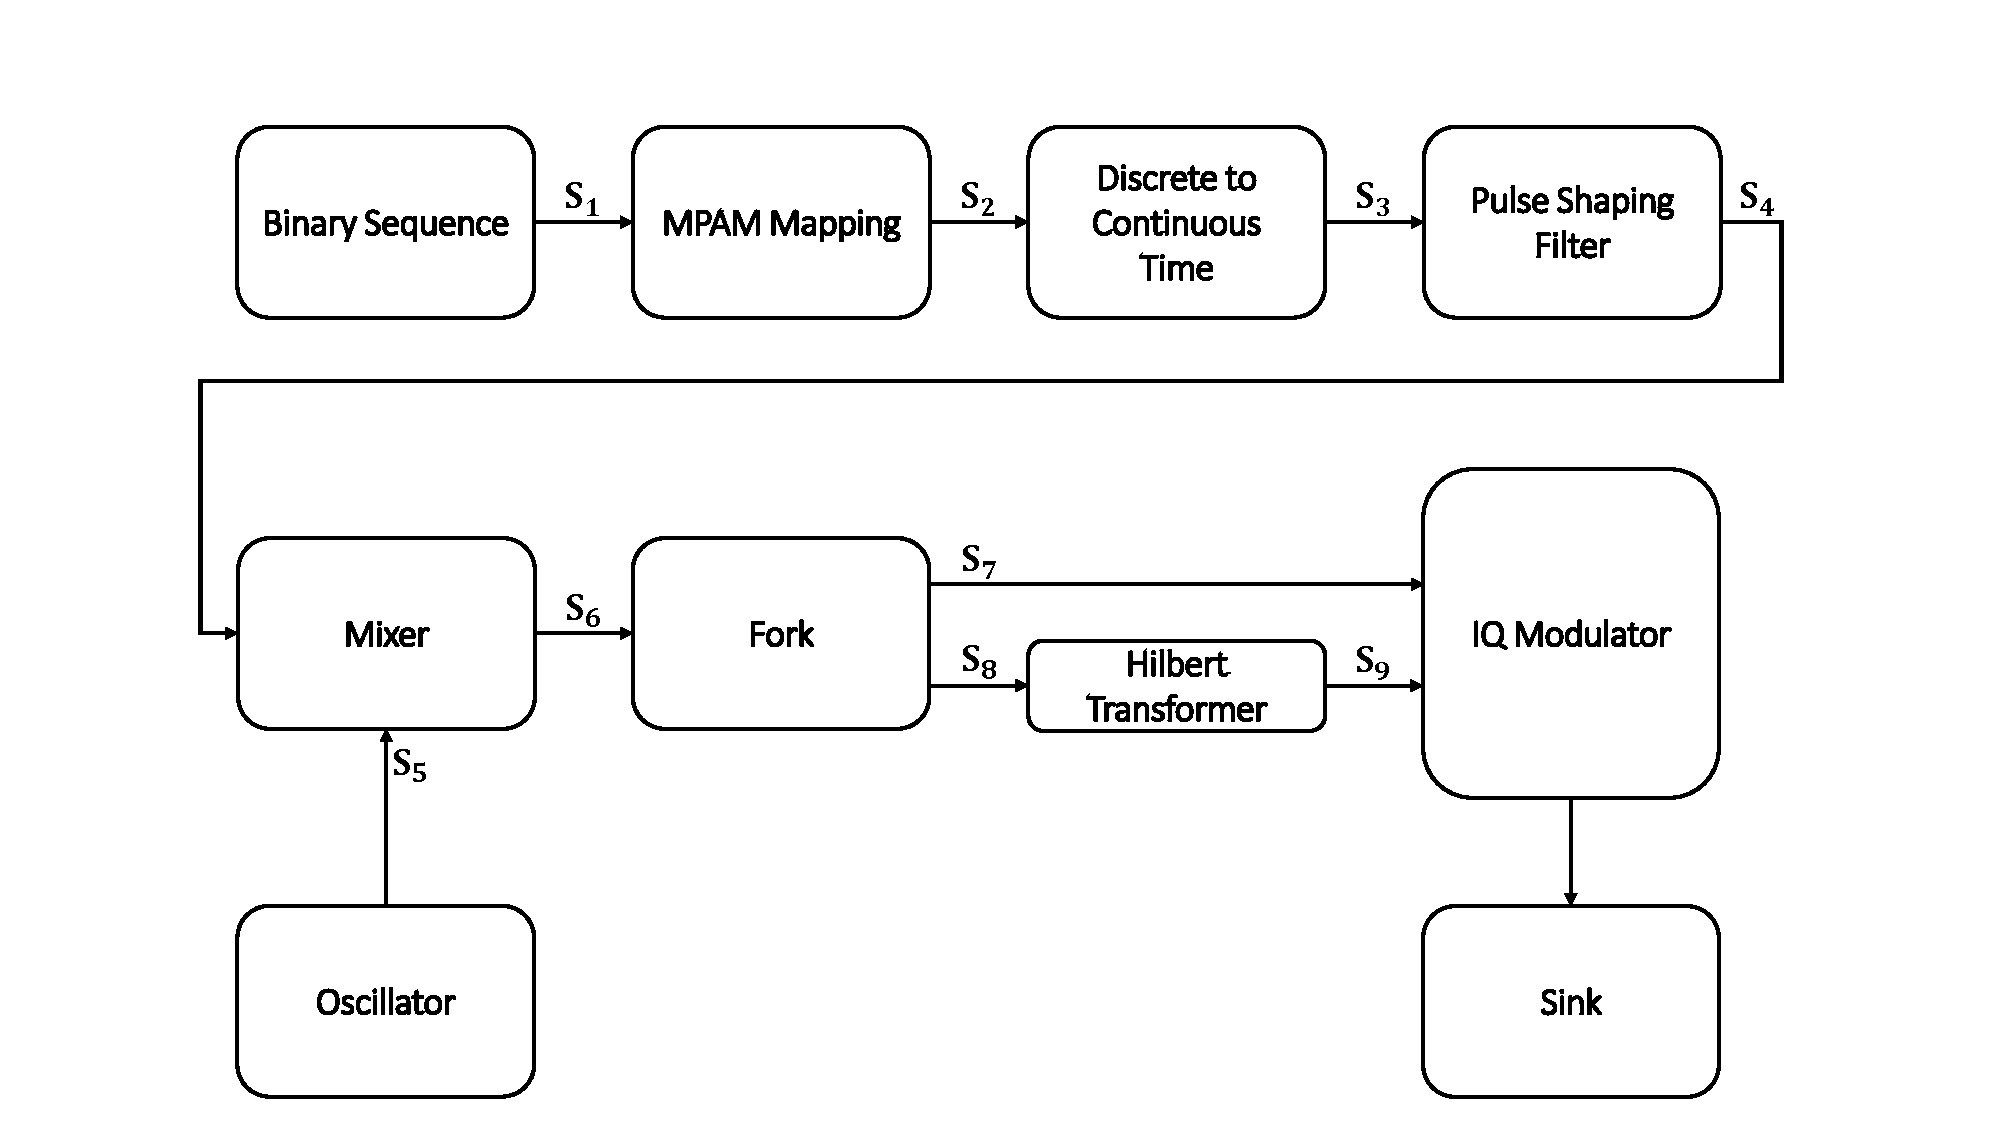
\includegraphics[width=1.0\textwidth, height=9cm]{./sdf/simplified_coherent_receiver/figures/Simulation_setup_Tx.pdf}
	\caption{Transmitter simulation setup}\label{Simulation_setup_Tx}
\end{figure}

\subsubsection{Rx side}
At the receiver end (Figure \ref{Simulation_setup_Rx}), to ensure minimum phase condition, an LO $A_0exp(i\pi Bt)$ added to the information carrying signal $A_s(t)$ using the frequency selective coupler to avoid signal and LO loss. This implementation accommodates polarization multiplexing and eliminates the need of optical hybrid. The minimum phase signal $A(t)$ applied to the single photo-detector for direct-detection which will generate photo current proportional to its intensity $I(t)=|A(t)|^2$ (assuming proportionality constant to be 1). From the amplitude data generated by single photo-detector, full reconstruction of the complex envelope carried out by the Kramers-Kronig algorithm. The availability of the complex signal at the end of reconstruction makes KK-PAM scheme equivalent to a coherent receiver which allows compensation of chromatic dispersion digitally. 

\begin{figure}[h]
	\centering
	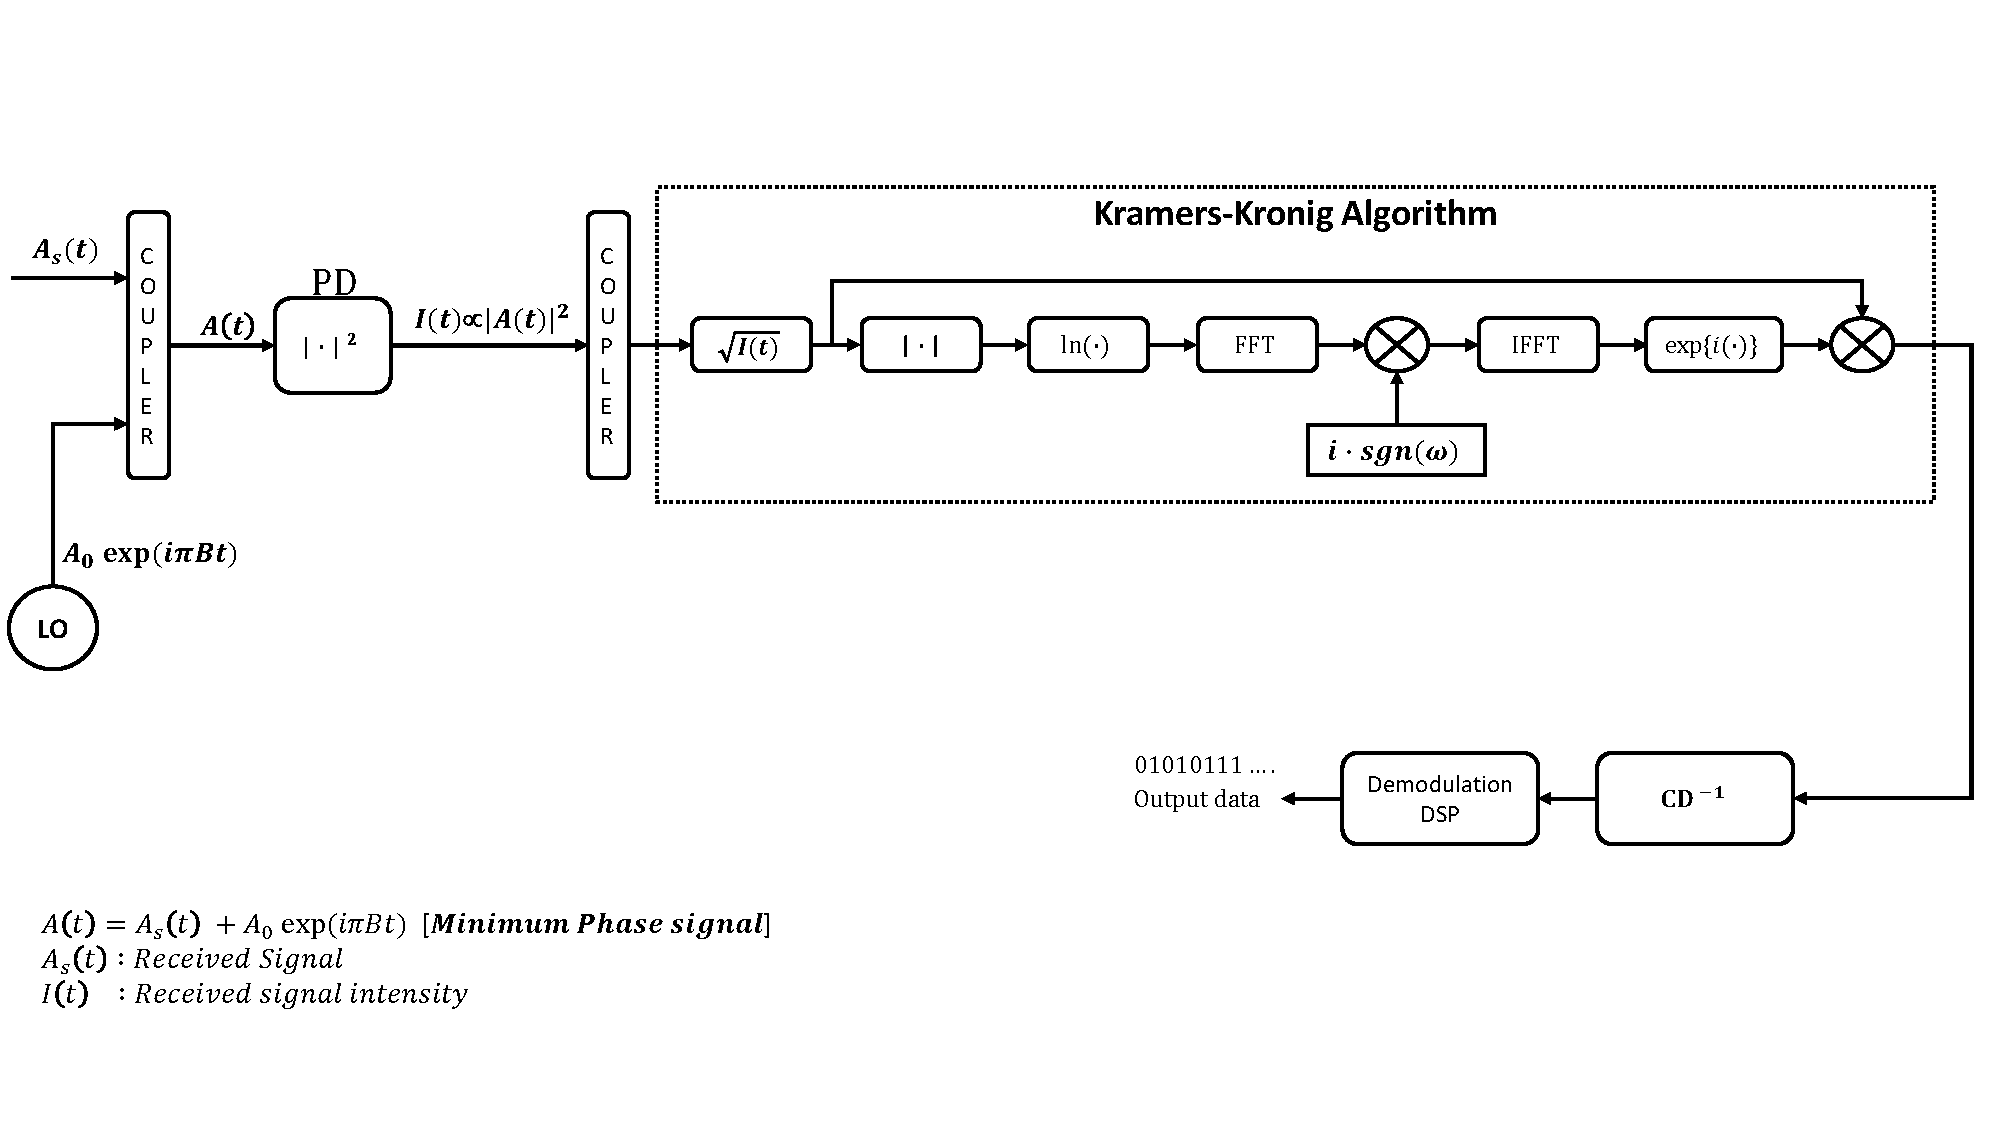
\includegraphics[width=1.0\textwidth, height=10cm]{./sdf/simplified_coherent_receiver/figures/Simulation_setup_Rx.pdf}
	\caption{Receiver simulation setup}\label{Simulation_setup_Rx}
\end{figure}


\subsection{Experimental set-up}
If an optical signal received together with a CW tone at the band edge such that it satisfies the minimum phase condition, then its full complex signal can be recovered after direct-detection by using KK algorithm. The principle can be extended to the dual-polarization signals through a polarization diversity transceiver set-up. As shown in the Figure \ref{Practical_setup_TxRx}, the PDM received signal first spitted by a polarization beam splitter (PBS). Each polarization is combined with an LO tapped from the transmit laser. The laser's wavelength and power are set to ensure that the received signal should satisfy the minimum phase condition. After direct-detection, Kramers-Kronig algorithm is performed on each polarization separately to recover full complex signal. After compensation of the chromatic dispersion, stokes parameter based polarization demux. algrithm can be applied to recover PDM signals.     

\begin{figure}[h]
	\centering
	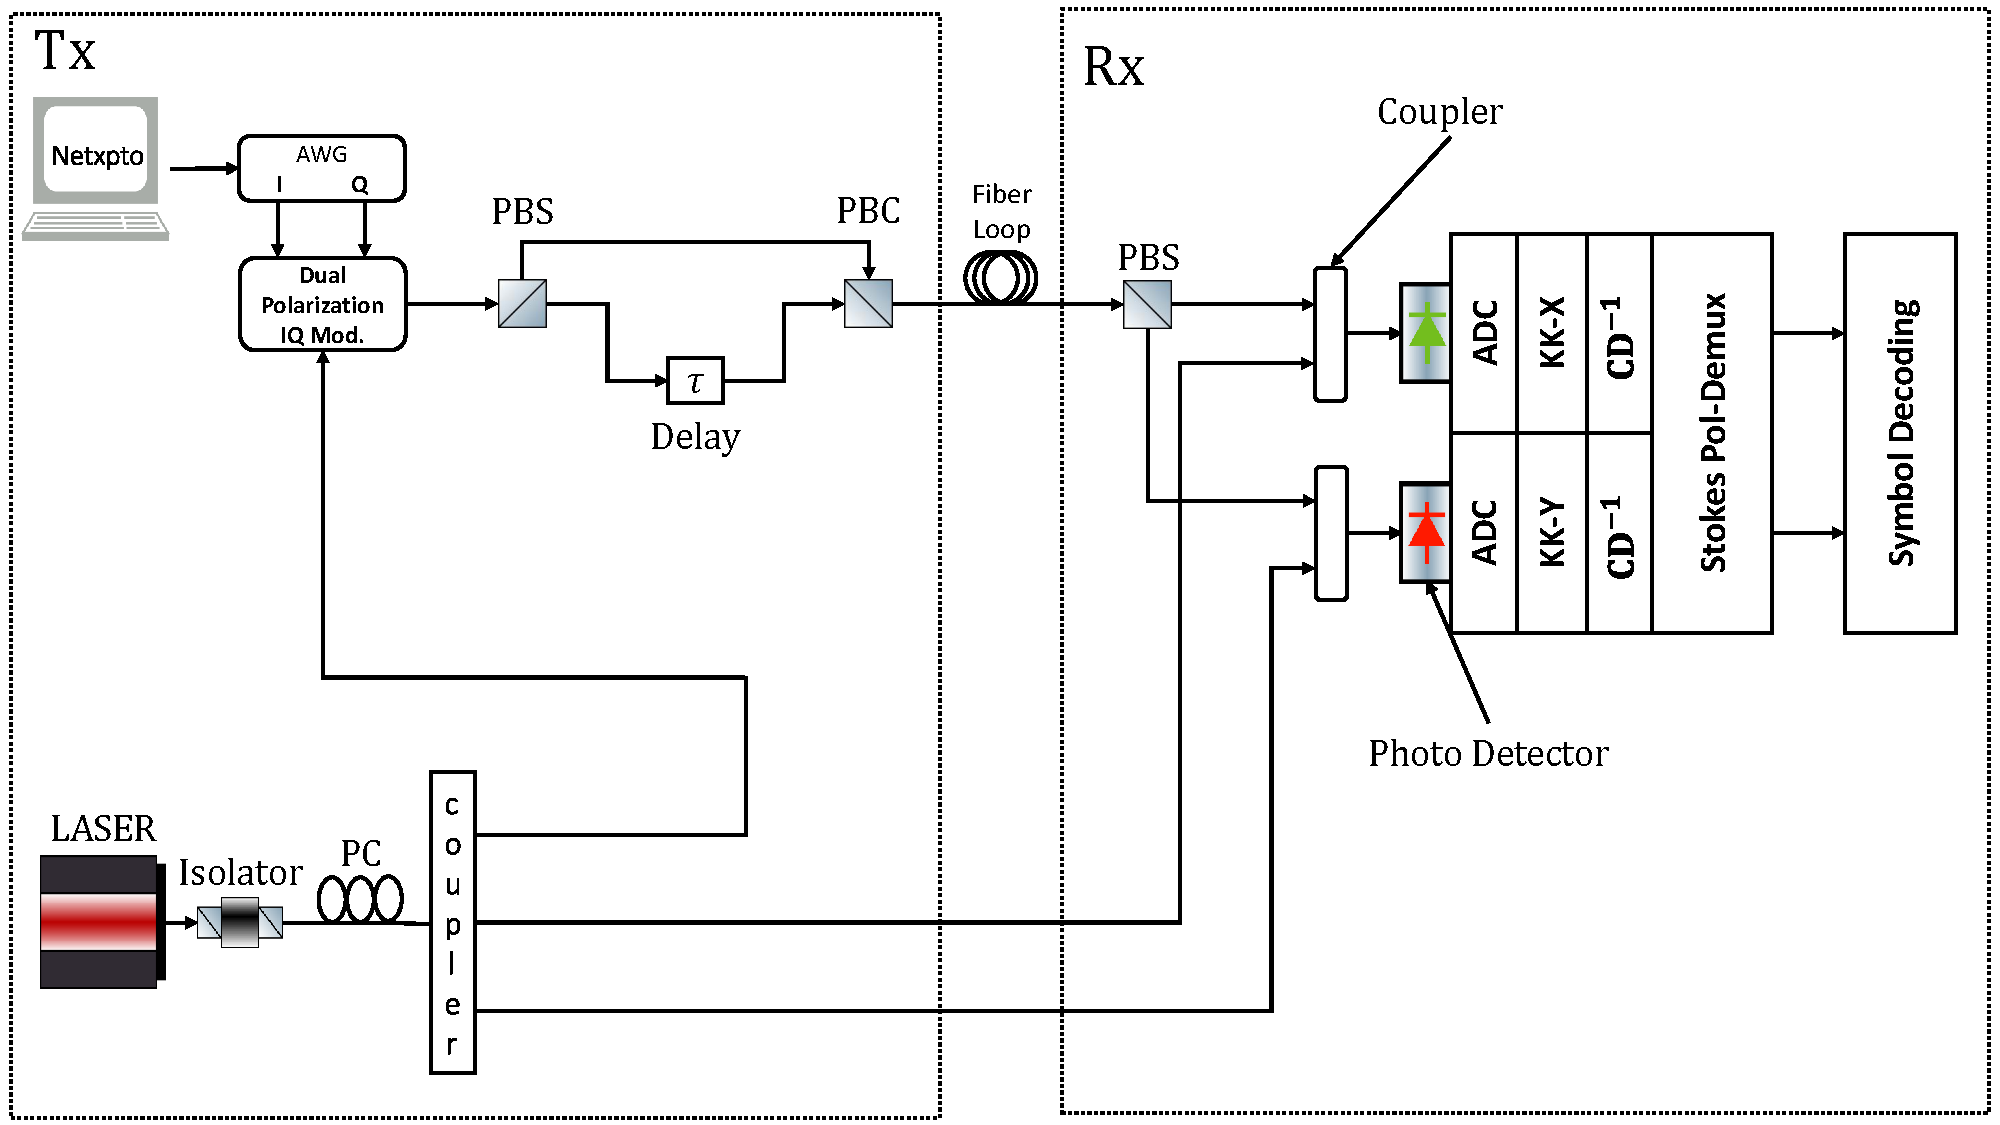
\includegraphics[width=1.0\textwidth, height=8cm]{./sdf/simplified_coherent_receiver/figures/Practical_setup_TxRx.pdf}
	\caption{PDM Kramers-Kronig receiver experimental setup}\label{Practical_setup_TxRx}
\end{figure}



\begin{thebibliography}{9}
	\bibitem{latexcompanion}
	Antonio Mecozzi, Cristian Antonelli, and Mark Shtaif.
	\textit{Kramers-Kronig Coherent Receiver}.
	Optica, vol.3, no.11, 2016, p.1220., doi:10.1364/optica.3.001220.
	
	\bibitem{latexcompanion}
	Antonio Mecozzi.
	\textit{Retrieving the full optical response from amplitude data by Hilbert transform}. Opt. Comm. 282, 4183-4187.
	
	\bibitem{latexcompanion}
	Antonio Mecozzi.
	\textit{A necessary and sufficient condition for minimum phase and implication of phase retrieval}. arXiv:1606.04861.
\end{thebibliography}










\subsubsection{\textbf{APPENDICES}}
%%%%%%%%%%%%%%%%%%%%%%%%%%%%%%%%%%%%%%%%%%%%%%%%%%%%%%%%%%%%%%%%%%%%%%%%%%%%%%%%%%%%%%%%%%%%%%%%%%%%%%%%%%
\textbf{Appendix A : Hilbert Transform}\\
If we consider a filter $H(\omega)$, described in Figure \ref{Hilbert_Transformer}, that has a unity magnitude response for all frequencies. Also, the phase response is $-\pi/2$ for all positive frequencies and $\pi/2$ for negative frequencies. The transfer function of this filter is,
\begin{equation}
\begin{split}
H(i\omega)=-isgn(\omega)
\end{split}
\label{}
\end{equation}
\begin{figure}[h]
	\centering
	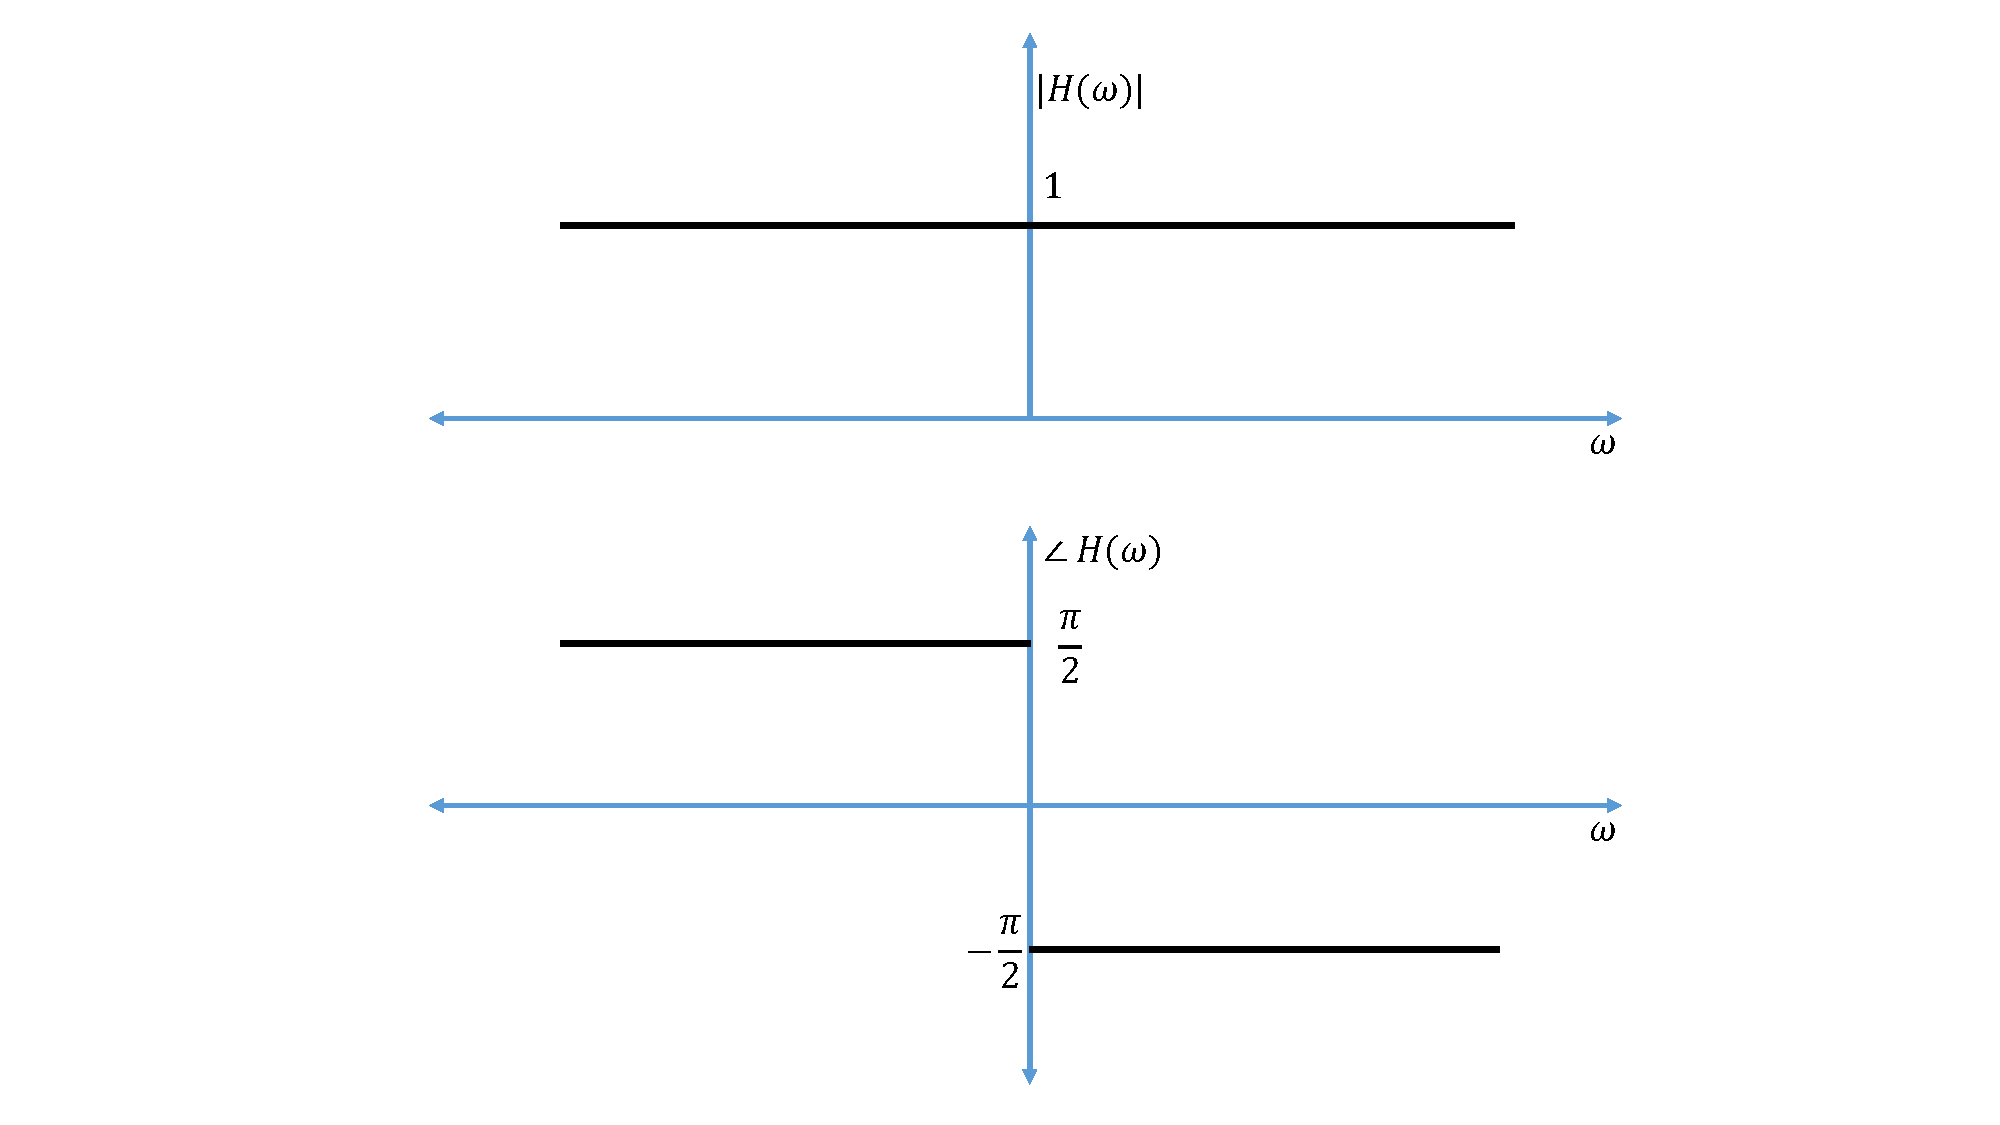
\includegraphics[width=1.0\textwidth, height=8cm]{./sdf/simplified_coherent_receiver/figures/HT.pdf}
	\caption{Magnitude and phase of Hilbert transformer}\label{Hilbert_Transformer}
\end{figure}
Therefore, we can term it as a wideband phase shift network. The inpulse response of this filter can be given as,
\begin{equation}
\begin{split}
h(t)&=\mathcal{F}^{-1}[H(i\omega)]\\
	&=-i\mathcal{F}^{-1}[sgn(\omega)]\\
	&=-i\bigg(\frac{i}{\pi t}\bigg)\\
	&=\frac{1}{\pi t}
\end{split}
\label{}
\end{equation}
When this filter driven by an arbitrary signal $s(t)$, the filter produces the output as,
\begin{equation}
\begin{split}
\hat{s}(t)&=s(t) * h(t)\\
		  &=\int_{-\infty}^{\infty} \dfrac{s(u)}{\pi(t-u)}du\\
\end{split}
\label{}
\end{equation}
The function $\hat{s}(t)$ is called the Hilbert transform if $s(t)$. Note that
\begin{equation}
\begin{split}
\mathcal{F}[\hat{h}(t)]=H(\omega)S(\omega)=-isgn(\omega)S(\omega)
\end{split}
\label{}
\end{equation}
In conclusion, if we convolve any time domain signal with $\frac{1}{\pi t}$ then it will give us Hilbert transformed signal in time domain. Similarly, from the convolution property of the Fourier transform, if we multiply $-isgn(\omega)$ with any frequency domain signal $S(\omega)$ then it'll give us Hilbert transformed signal in frequency domain.
%%%%%%%%%%%%%%%%%%%%%%%%%%%%%%%%%%%%%%%%%%%%%%%%%%%%%%%%%%%%%%%%%%%%%%%%%%%%%%%%%%%%%%%%%%%%%%%%%%%%%%%%%%
\\
\\
\textbf{Appendix B : Single Sideband Signal (SSB) generation}\\
In this section, we'll discuss the brief idea of generating SSB signal using Hilbert transform method. To understand this, we may express signal $u(t)$ as a summation of the two complex-valued functions.
\begin{equation}
s(t)=\dfrac{1}{2}[s(t)+j\hat{s}(t)]+\dfrac{1}{2}[s(t)-j\hat{s}(t)]
\label{}
\end{equation}
where, the term $\dfrac{1}{2}[s(t)+j\hat{s}(t)]$ is the analytical representation of the signal $s(t)$ (from Equation \ref{Analytical signal}). Another term represents the complex conjugate $\dfrac{1}{2}[s(t)-j\hat{s}(t)]$ of this analytical signal. Such representation of the signal ${s_a}(t)$ and ${s_a^*}(t)$ divide the signal into non-negative frequency component and non-positive frequency component respectively. Alternatively, we can write it as,
\begin{equation}
\dfrac{1}{2}{S_a}(f) = \begin{cases}
S(f) &\text{for $f>0$}\\
0    &\text{for $f<0$}\\
\end{cases}
\end{equation}
where ${S_a}(f)$ and ${S}(f)$ are the Fourier transform of ${t_a}(t)$ and ${s}(t)$ respectively. The frequency translated version of ${S_a}(f-f_0)$ contains only one side (positive) of ${S}(f)$ and hence it is called single sideband signal ${s_ssb}(t)$,
\begin{equation}
{F}^{-1}\{S_a(f-f_0)\}={s_a}(t) e^{j2\pi f_0 t}={s_{ssb}}(t)+j{\hat{s}_{ssb}(t)}
\end{equation}
Therefore, from the Euler's formula,
\begin{equation}
\begin{split}
{s}_{ssb}(t)&=Re\{s_a(t)  e^{j2\pi f_0 t}\}\\
&=Re\{[s(t)+j\hat{s}(t)] [cos(2\pi f_0t)+jsin(2\pi f_0t)]\}\\
&=s(t)cos(2\pi f_0t)-\hat{s}(t)sin(2\pi f_0t)
\end{split}
\label{USB_SSB}
\end{equation}
This Equation \ref{USB_SSB} displays the mathematical modeling of the upper sideband SSB signal. Similarly, we can generate lower sideband SSB signal by,
\begin{equation}
{s}_{ssb}(t)=s(t)cos(2\pi f_0t)+\hat{s}(t)sin(2\pi f_0t)
\label{LSB_SSB}
\end{equation}\\
%%%%%%%%%%%%%%%%%%%%%%%%%%%%%%%%%%%%%%%%%%%%%%%%%%%%%%%%%%%%%%%%%%%%%%%%%%%%%%%%%%%%%%%%%%%%%%%%%%%%%%%%%%
\\
\textbf{Appendix C : Kramers-Kronig relationship}\\
%\subsubsection{Kramers Kronig Relation}
Suppose we have a SSB signal $u(t)$ described as,
\begin{equation}
E_s(t)=E_{s,r}(t)+iE_{s,i}(t)
\label{Eq:5.31}
\end{equation}
In the equation \ref{Eq:5.22}, the real and imaginary parts $E_{s,r}(t)$ and $E_{s,i}(t)$ are related through the Kramers-Kronig relation with each other. An intuitive way to analyze the relation is based on expressing its Fourier transform $E_s(\omega)$ as follows,
\begin{equation}
E_s(\omega)=\dfrac{1}{2}[1+sgn(\omega)]E_s(\omega)
\label{Eq:5.23}
\end{equation}
The equation \ref{Eq:5.23} follows the SSB signal condition $E_s(\omega)=0$ for $\omega<0$. Further, simplification0n of the signal can be summarized as follows:
\begin{equation}
\begin{split}
E_s(\omega)&=\dfrac{1}{2}[1+sgn(\omega)]E_s(\omega)\\
&=\dfrac{1}{2}E_s(\omega)+\dfrac{1}{2}sgn(\omega)E_s(\omega)
\end{split}
\label{Eq:5.33}
\end{equation}
Taking inverse Fourier transform of the equation \ref{Eq:5.33},
\begin{equation}
\begin{split}
{E_s}(t)&=IFT\{E_s(\omega)\}\\
&=\dfrac{1}{2}{E_s}(t)+\underline{\dfrac{1}{2}[IFT\{sgn(\omega)\} \circledast {E_s}(t)]}
\end{split}
\label{Eq:5.34}
\end{equation}
The underlined term in Equation \ref{Eq:5.34} displays that multiplication in frequency domain converted into the convolution in the time domain. Further, IFT of the function $sgn(\omega)$ given as $(-i/\pi t)$. As a consequences, we can further simplify our equation as,
\begin{equation}
\begin{split}
{E_s}(t)&=\dfrac{1}{2}{E_s}(t)+\frac{1}{2}\bigg[\frac{i}{\pi t} \circledast {E_s}(t) \bigg]\\
\frac{{E_s}(t)}{2} &=\frac{1}{2}\bigg[\frac{i}{\pi t} \circledast {E_s}(t) \bigg]\\
{E_s}(t) &=i\bigg[\frac{1}{\pi t} \circledast {E_s}(t) \bigg]\\
{E_s}(t) &=\frac{i}{\pi} p.v. \int_{-\infty}^{\infty} \frac{E_s(t')}{t-t'} dt' 
\end{split}
\label{Eq:5.35}
\end{equation}
Using Equation \ref{Eq:5.31} into Equation \ref{Eq:5.35},
\begin{equation}
\begin{split}
E_{s,r}(t)+iE_{s,i}(t) &=\frac{i}{\pi} p.v. \int_{-\infty}^{\infty} \frac{E_s(t')}{t-t'} dt' 
\end{split}
\label{Eq:5.36}
\end{equation}
Therefore,
\begin{equation}
\begin{split}
E_{s,r}(t)+iE_{s,i}(t) &=\frac{i}{\pi} p.v. \int_{-\infty}^{\infty} \frac{E_{s,r}(t')+iE_{s,r}(t')}{t-t'} dt' \\
E_{s,r}(t)+iE_{s,i}(t)&=-\frac{1}{\pi} p.v. \int_{-\infty}^{\infty} \frac{E_{s,i}(t')}{t-t'} dt' + \frac{i}{\pi} p.v. \int_{-\infty}^{\infty} \frac{E_{s,r}(t')}{t-t'} dt'
\end{split}
\label{Eq:5.37}
\end{equation}
which leads to,
\begin{equation}
\begin{split}
E_{s,r}(t) &=-\frac{1}{\pi} p.v. \int_{-\infty}^{\infty} \frac{E_{s,i}(t')}{t-t'} dt' \\
E_{s,i}(t) &=\frac{1}{\pi} p.v. \int_{-\infty}^{\infty} \frac{E_{s,r}(t')}{t-t'} dt' \\
\end{split}
\label{Eq:5.38}
\end{equation}
%%%%%%%%%%%%%%%%%%%%%%%%%%%%%%%%%%%%%%%%%%%%%%%%%%%%%%%%%%%%%%%%%%%%%%%%%%%%%%%%%%%%%%%%%%%%%%%%%%%%%%%%%%
\\
\\
\textbf{Appendix D : Phase reconstruction from minimum phase SSB signal}\\
Given function $E(t)=E_{s}(t)+\bar{E}$ never encircles the origin for $t\in(-\infty,\infty)$. if we define,
\begin{equation}
G(t)=log\bigg[\dfrac{E(t)}{\bar{E}}\bigg]
\label{Eq 5.39}
\end{equation} 
then $G(\omega)$, the spectrum of $G(t)$, is such that $G(\omega)=0$ for $\omega<0$. Under the hypothesis stated by Equation \ref{Eq:5.17},we can write $G(t)$ as,
\begin{equation}
\begin{split}
G(t) &=\frac{i}{\pi} p.v. \int_{-\infty}^{\infty} \frac{G(t')}{t-t'} dt' 
\end{split}
\label{Eq 5.40}
\end{equation}
From the equations \ref{Eq 5.39} and \ref{Eq 5.40},
\begin{equation}
\begin{split}
log|E(t)|-log|\bar{E}|+i[\phi(t)-\bar{\phi}] &=\frac{i}{\pi} p.v. \int_{-\infty}^{\infty} \frac{log|E(t)|-log|\bar{E}|}{t-t'} dt' + \frac{1}{\pi} p.v. \int_{-\infty}^{\infty} \frac{\phi(t)-\bar{\phi}}{t-t'} dt' 
\end{split}
\label{Eq 5.41}
\end{equation}
Comparing Imaginary part of Equation \ref{Eq 5.41},
\begin{equation}
\begin{split}
\phi(t)-\bar{\phi} &= + \frac{1}{\pi} p.v. \int_{-\infty}^{\infty} \frac{log|E(t)|-log|\bar{E}|}{t-t'} dt'\\
\end{split}
\label{Eq 5.42}
\end{equation}
In equation \ref{Eq 5.42}, $\frac{1}{\pi} p.v. \int_{-\infty}^{\infty} \frac{log|\bar{E}|}{t-t'} dt'=0$ which leads to,
\begin{equation}.
\begin{split}
\phi(t) &= \bar{\phi} + \frac{1}{\pi} p.v. \int_{-\infty}^{\infty} \frac{log|E(t)|}{t-t'} dt'\\
\phi(t) &= \bar{\phi} + \frac{1}{2\pi} p.v. \int_{-\infty}^{\infty} \frac{log|E(t)|^2}{t-t'} dt'\\
\end{split}
\label{Eq 5.43}
\end{equation}
%%%%%%%%%%%%%%%%%%%%%%%%%%%%%%%%%%%%%%%%%%%%%%%%%%%%%%%%%%%%%%%%%%%%%%%%%%%%%%%%%%%%%%%%%%%%%%%%%%%%%%%%%%
%%%%%%%%%%%%%%%%%%%%%%%%%%%%%%%%%%%%%%%%%%%%%%%%%%%%%%%%%%%%%%%%%%%%%%%%%%%%%%%%%%%%%%%%%%%%%%%%%%%%%%%%%%
\\
\textbf{Appendix E : SSB with graphical explanation}\\
This section describes the SSB signal generation using Hilbert transformation method (Phase Shift Method). Consider a message signal $m(t)$ with its frequency domain spectrum $M(F)$ as shown in Figure\ref{Original_baseband_signal}. From the Figure \ref{Original_baseband_signal}, we can see that both the side are scaled by factor '1' which means it represents the original signal.
\begin{figure}[h]
	\centering
	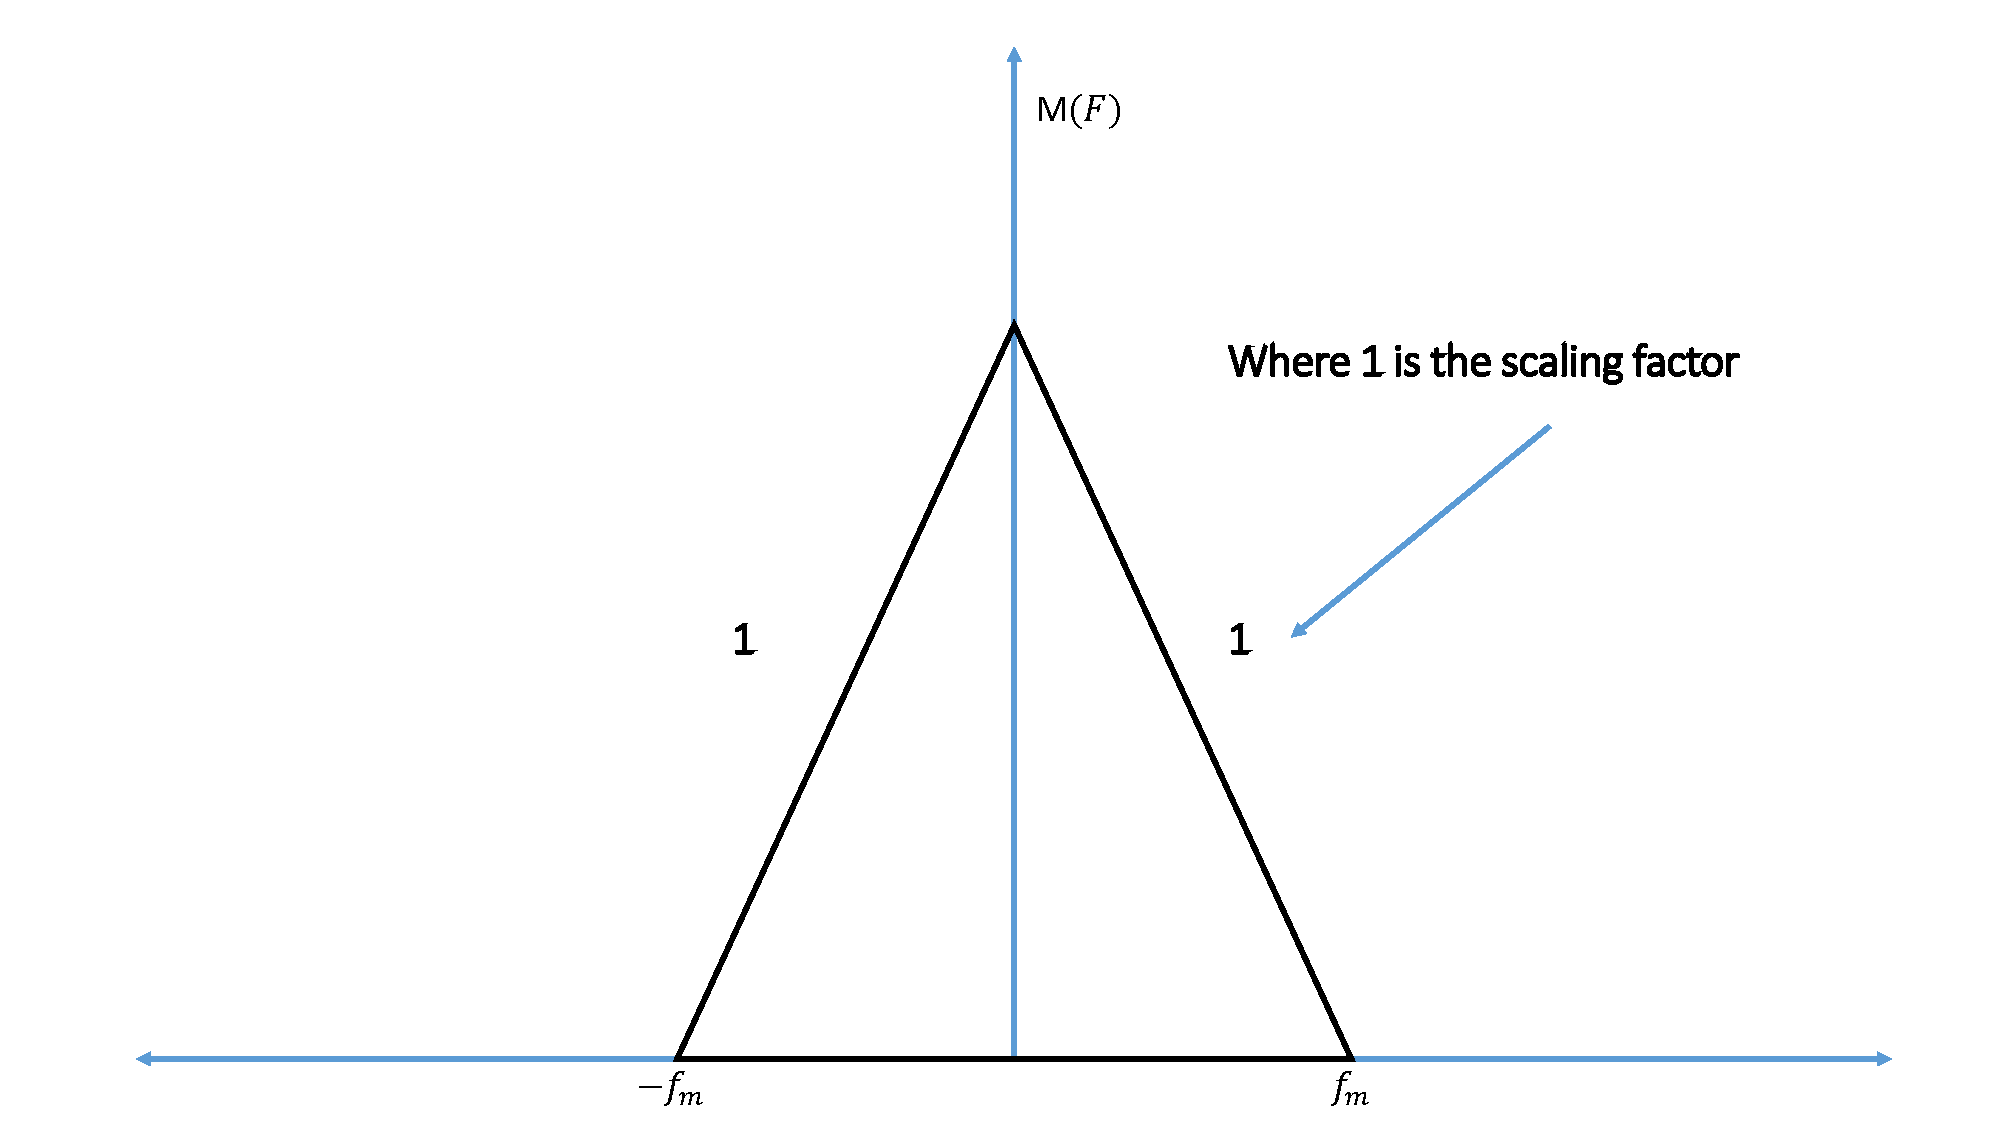
\includegraphics[width=0.6\textwidth, height=5cm]{./sdf/simplified_coherent_receiver/figures/SSB1.pdf}
	\caption{Original baseband signal}\label{Original_baseband_signal}
\end{figure}\\ 	
Now let's consider the modulated signal $x(t)$ given as,
\begin{equation}
x(t)=m(t) cos(2\pi f_c t)
\label{Eq:5.20}
\end{equation}
Frequency domain representation of the equation \ref{Eq:5.20} can be given as,
\begin{equation}
X(F)=\frac{1}{2}M(f-f_c)+\frac{1}{2}M(f+f_c)
\label{Eq:5.21}
\end{equation}
Here in equation \ref{Eq:5.21}, we can observe that each side band are scaled by $\dfrac{1}{2}$ on the frequency spectrum. Figure displays the frequency domain representation of the modulated signal $X(F)$.
\begin{figure}[h]
	\centering
	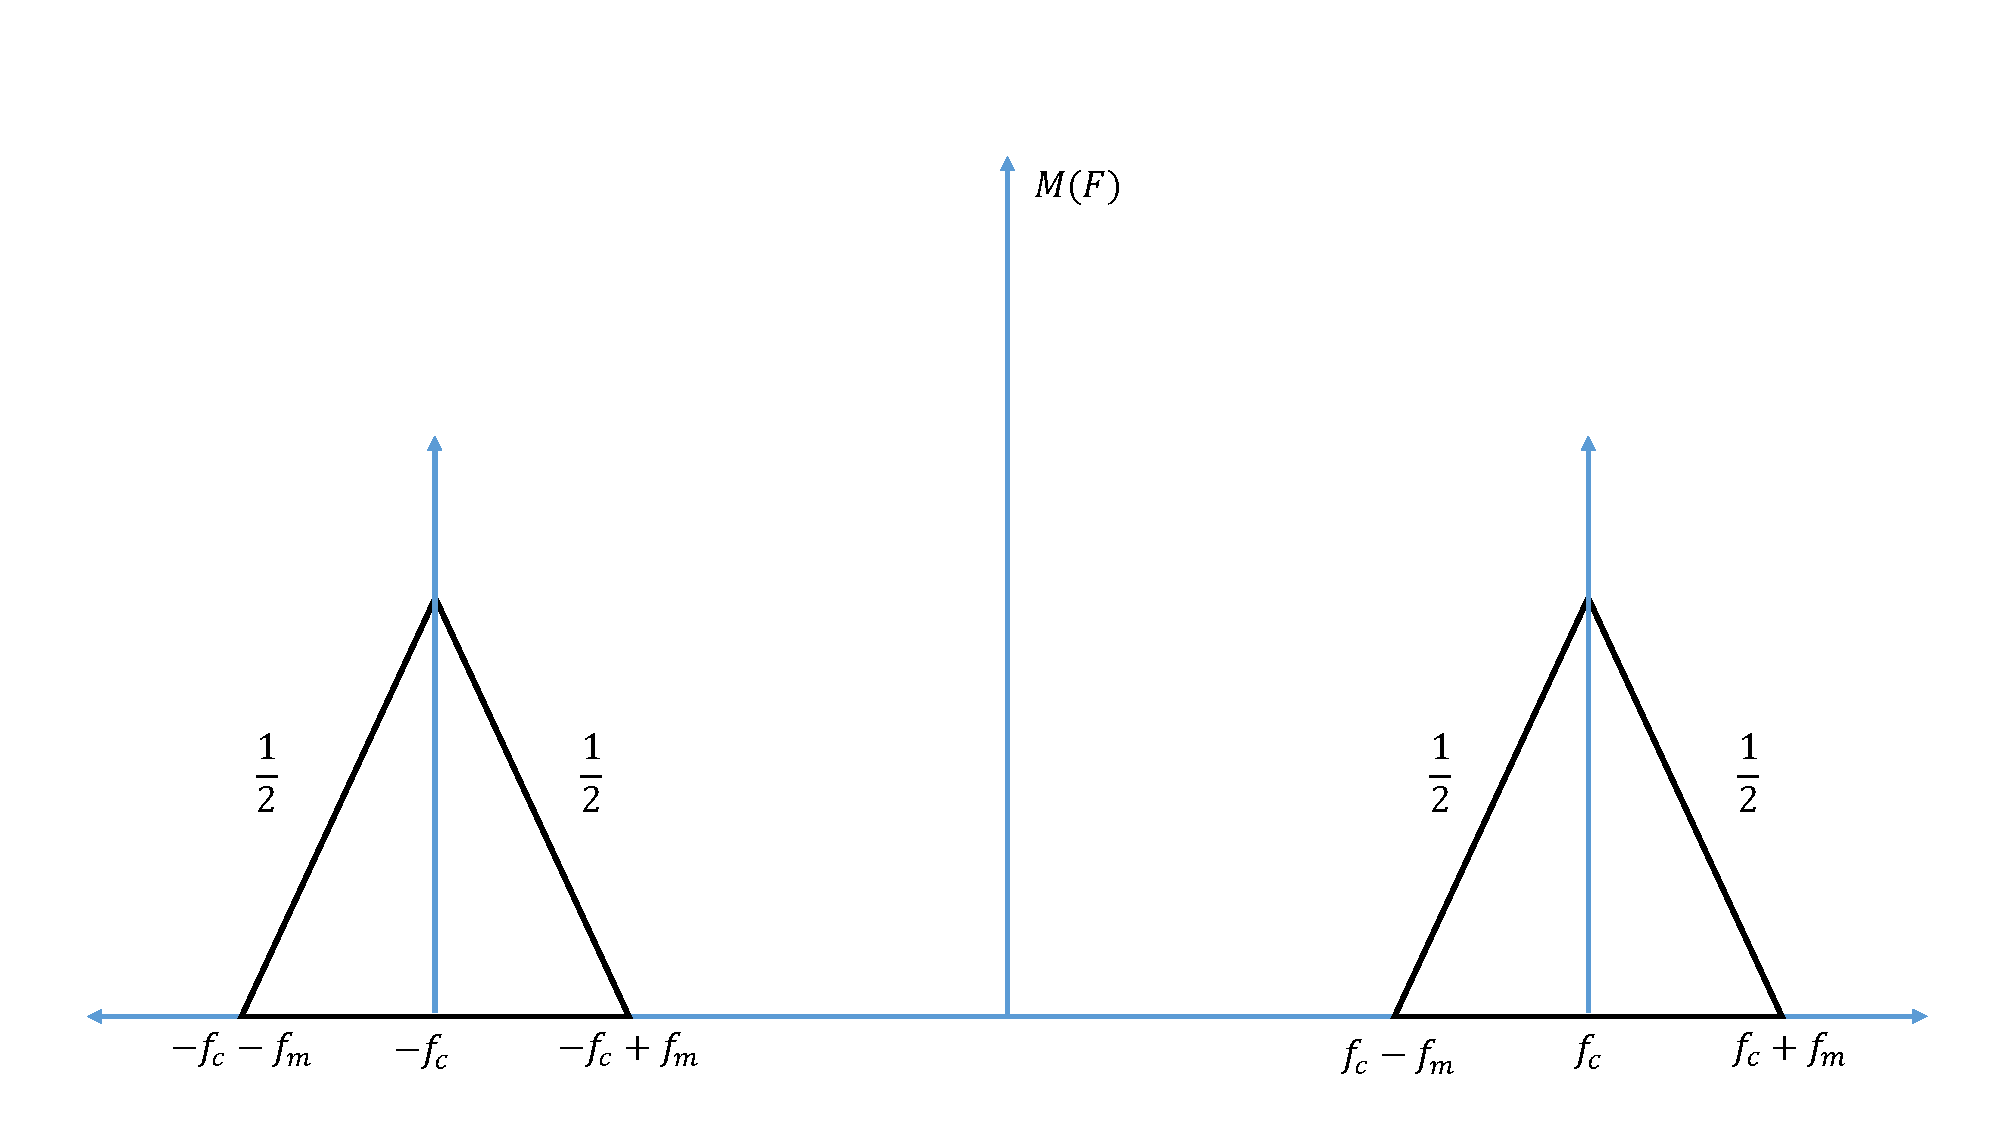
\includegraphics[width=1.0\textwidth, height=8cm]{./sdf/simplified_coherent_receiver/figures/SSB2.pdf}
	\caption{Original modulated signal}\label{Original_modulated_signal}
\end{figure}\\ 
Next, we will discuss something more interesting which is called as Hilbert transform of the original message signal $m(t)$. As we discussed earlier, in the frequency domain, the Hilbert transformed signal $\hat{M}(f)$ can be achieved by multiplying the Fourier transformed signal $M(F)$ with $[-i sgn(F)]$.
\begin{figure}[h]
	\centering
	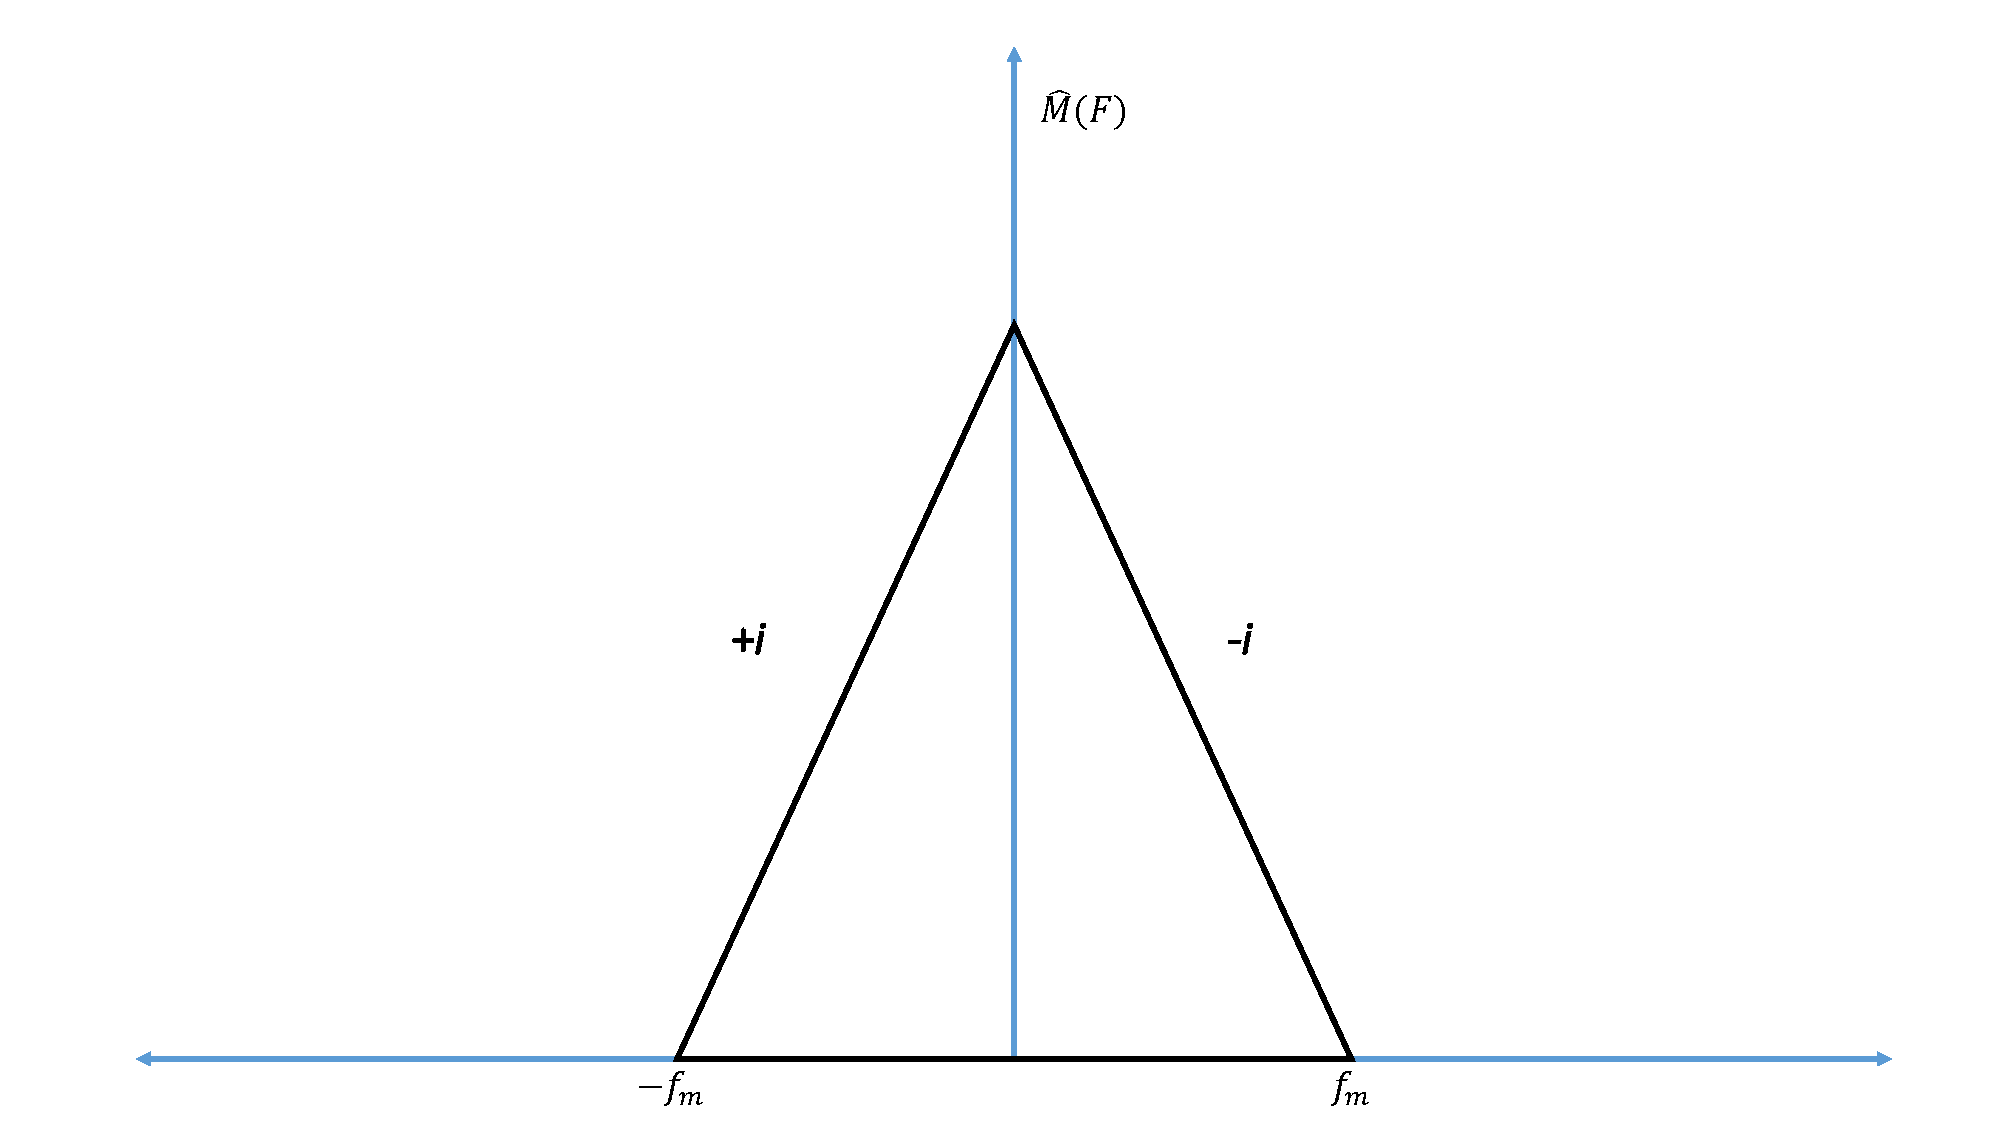
\includegraphics[width=0.6\textwidth, height=5cm]{./sdf/simplified_coherent_receiver/figures/SSB3.pdf}
	\caption{Hilbert transformed modulated signal}\label{Hilbert_Transformed_signal}
\end{figure}
Suppose we modulate the Hilbert transformed message signal $\hat{m}(t)$  with the $sin(2\pi f_c t)$ (quadrature phase carrier), then we get the following results:

\begin{equation}
\begin{split}
{\hat{m}(t)} sin(2\pi f_c t)&={\hat{m}(t)}\frac{e^{i2\pi f_c t} - e^{-i2\pi f_c t} }{2}\\
&={\hat{m}(t)}\frac{e^{i2\pi f_c t}}{2} - {\hat{m}(t)}\frac{e^{-i2\pi f_c t}}{2}\\
&={\frac{\hat{M}(f-f_c)}{2i}}-{\frac{\hat{M}(f+f_c)}{2i}}\\
&={\frac{-i}{2}\hat{M}(f-f_c)}+{\frac{-i}{2}\hat{M}(f+f_c)}\\
\end{split}
\label{Eq:5.46}
\end{equation}
The detailed explanation of the equation \ref{Eq:5.46} has been given in the Figure \ref{Hilbert_Transformed_modulated_signal} and \ref{Hilbert_Final}. Figure \ref{Hilbert_Transformed_modulated_signal} displays the spectrum of the $\hat{M}(f+f_c)$ and $\hat{M}(f-f_c)$ for the positive and negative frequencies respectively. The final equation resolution of equation displays that both positive and negative side of the spectrum multiplied with $\frac{i}{2}$ and $\frac{-i}{2}$ respectively. Finally the spectrum of the signal ${\hat{m}(t)} sin(2\pi f_c t)$ can be given as Figure \ref{Hilbert_Final}.
\begin{figure}[h]
	\centering
	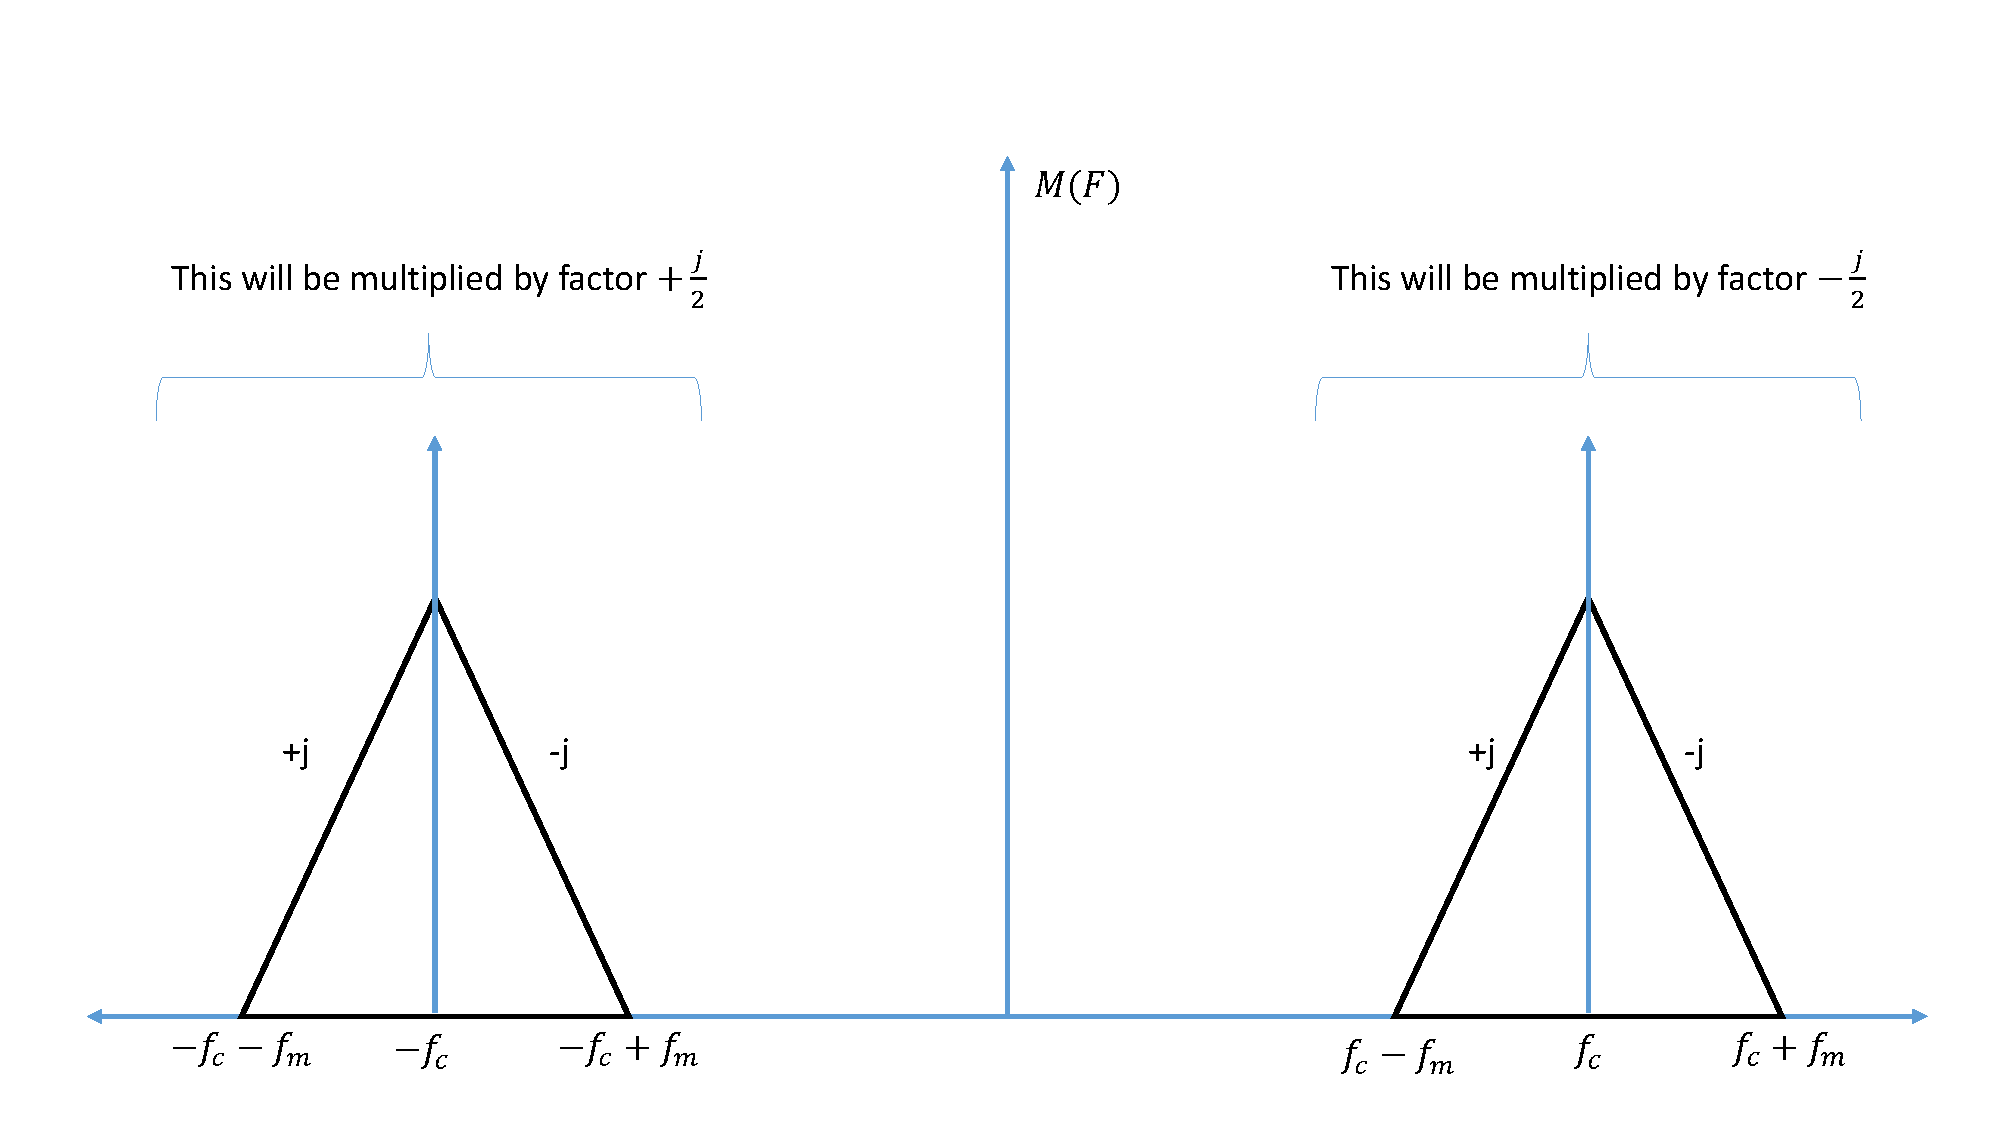
\includegraphics[width=1.0\textwidth, height=8cm]{./sdf/simplified_coherent_receiver/figures/SSB4.pdf}
	\caption{Hilbert transformed modulated signal}\label{Hilbert_Transformed_modulated_signal}
\end{figure}

\begin{figure}[h]
	\centering
	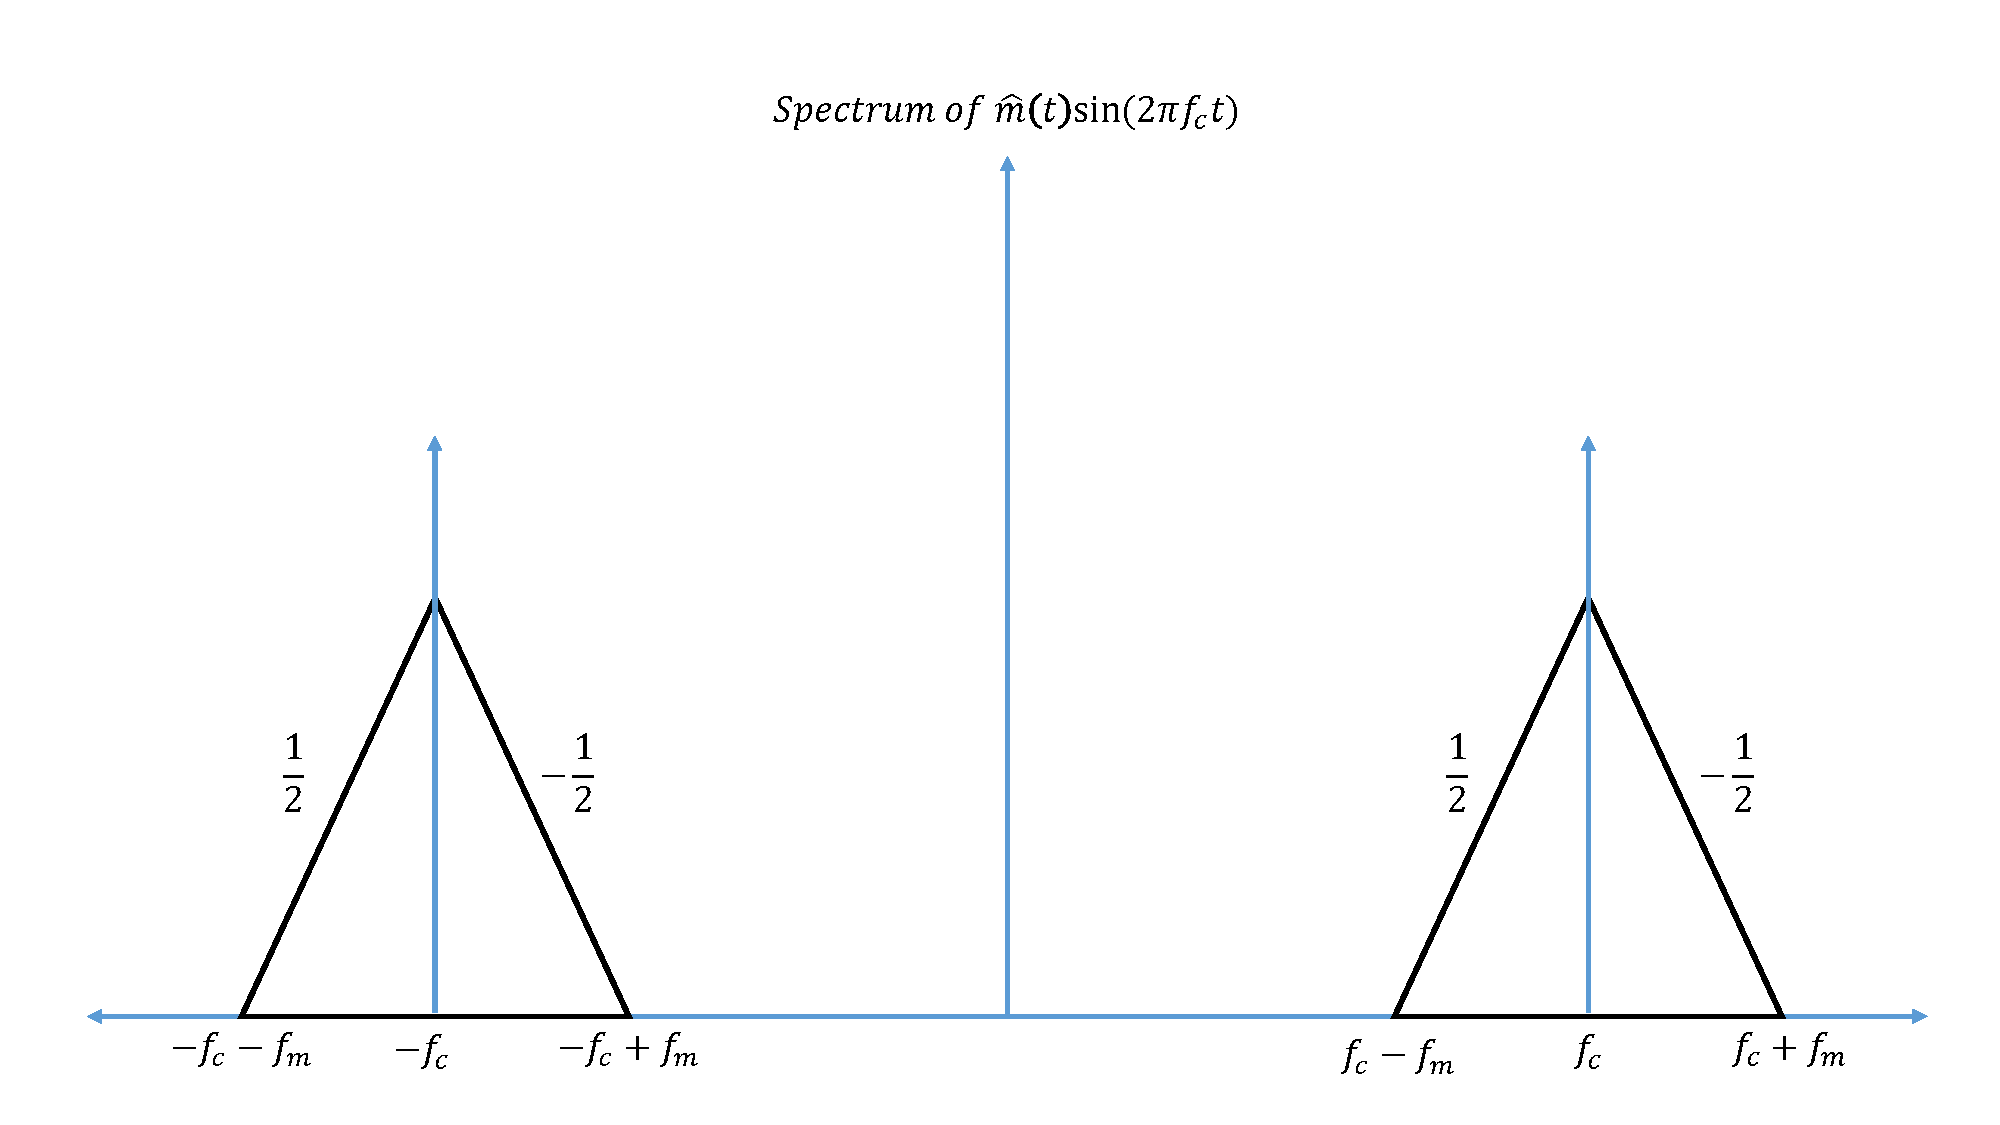
\includegraphics[width=1.0\textwidth, height=8cm]{./sdf/simplified_coherent_receiver/figures/SSB5.pdf}
	\caption{Hilbert transformed modulated signal}\label{Hilbert_Final}
\end{figure}

Further, summation of the two signals ${m(t)} cos(2\pi f_c t)$ and ${\hat{m}(t)} sin(2\pi f_c t)$ will generate the upper sideband SSB signal as follows,
\begin{equation}
u(t)={m(t)} cos(2\pi f_c t)-{\hat{m}(t)} sin(2\pi f_c t)
\label{5.23}
\end{equation}
From the above discussion, the spectrum of the Equation \ref{5.23} can be given by the Figure \ref{SSB_signal_spectrum}. Similarly, for the lower sideband SSB can be generated by Equation,
\begin{equation}
u(t)={m(t)} cos(2\pi f_c t)+{\hat{m}(t)} sin(2\pi f_c t)
\label{5.24}
\end{equation}
\begin{figure}[h]
	\centering
	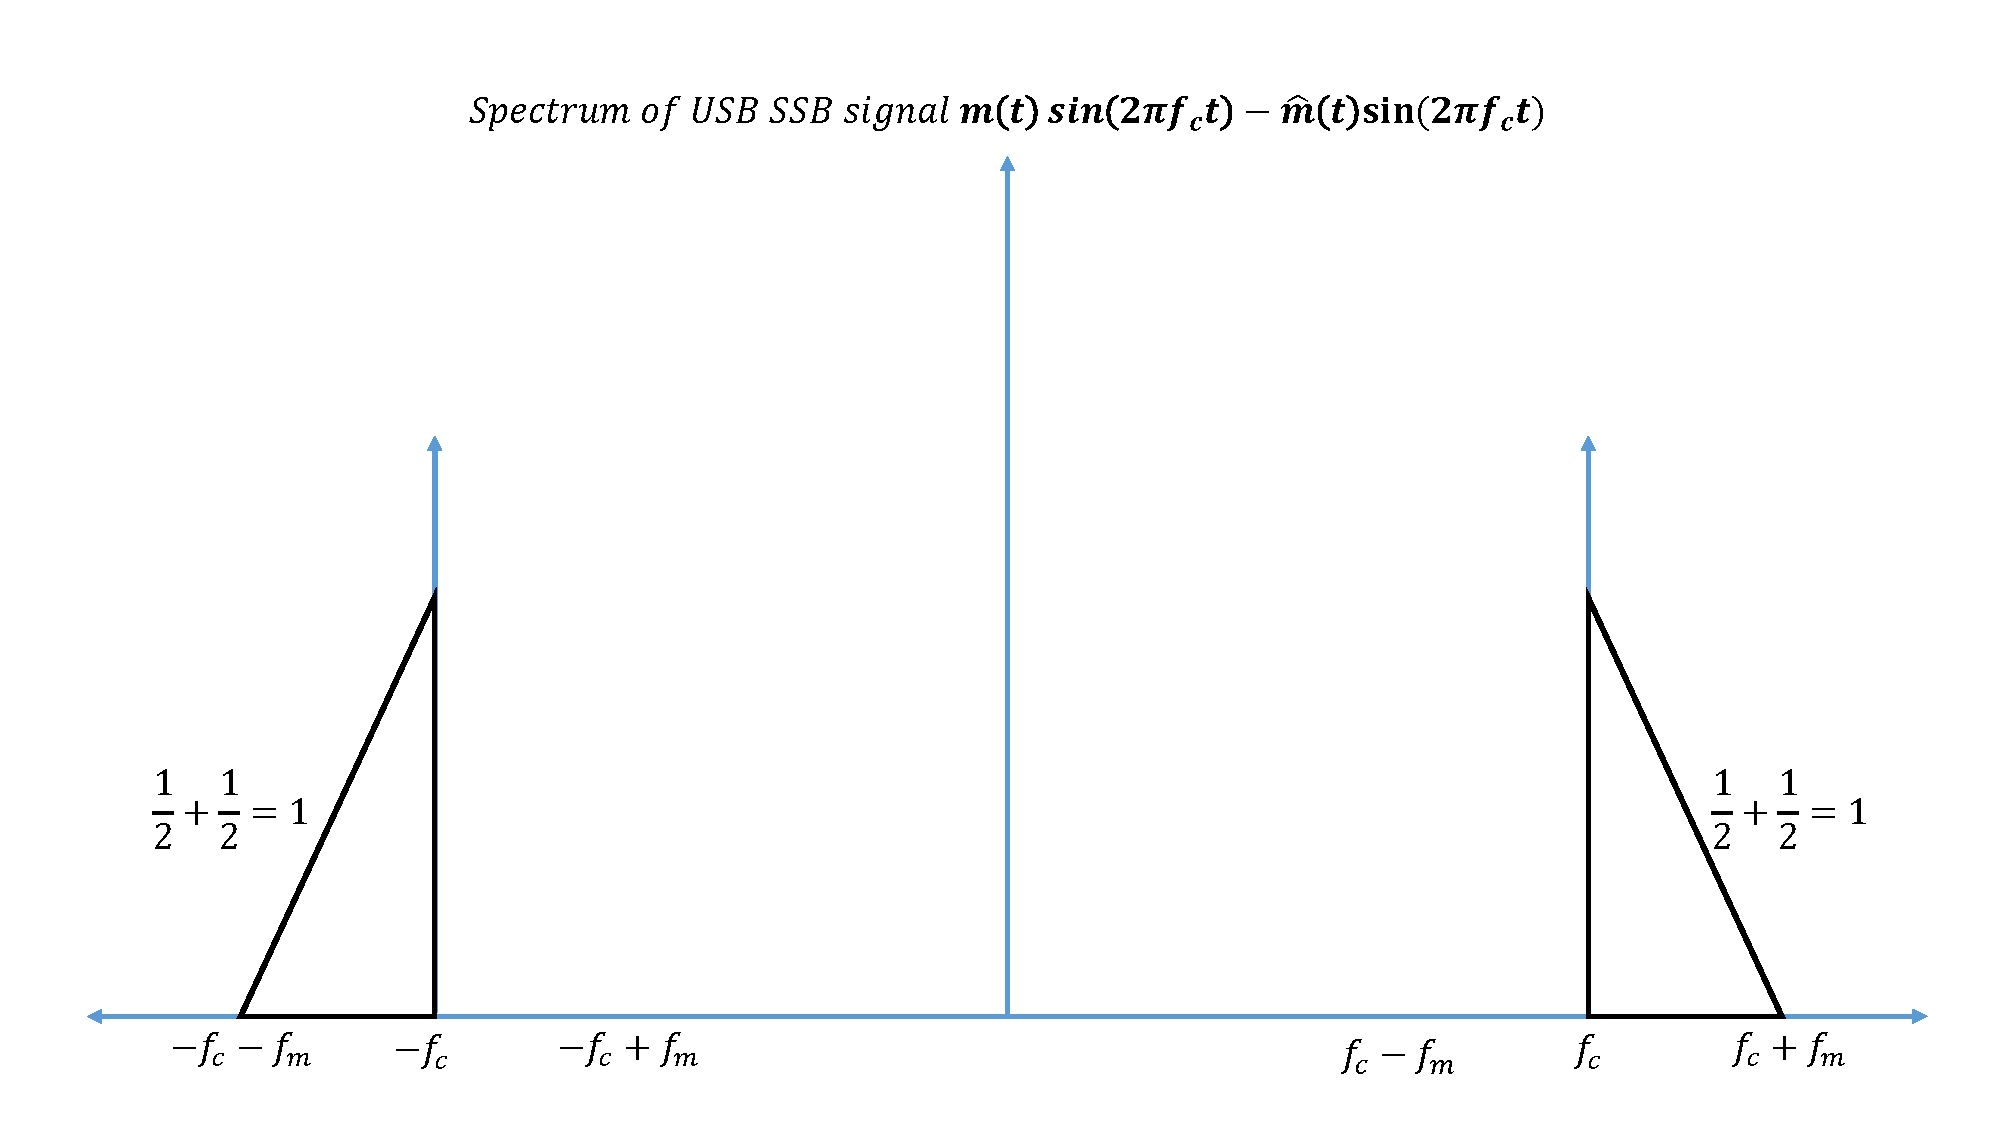
\includegraphics[width=1.0\textwidth, height=8cm]{./sdf/simplified_coherent_receiver/figures/SSB6.pdf}
	\caption{SSB signal spectrum}\label{SSB_signal_spectrum}
\end{figure}

\subsubsection{Kramers Kronig Relation}
Suppose we have a SSB signal $u(t)$ described as,
\begin{equation}
u(t)=u_r(t)+iu_i(t)
\label{Eq:5.22}
\end{equation}
In the equation \ref{Eq:5.22}, the real and imaginary parts $U_r(t)$ and $U_i(t)$ are related through the Kramers-Kronig relation with each other. An intuitive way to analyze the relation is based on expressing its Fourier transform $\tilde{U}(\omega)$ as follows,
\begin{equation}
\tilde{U}(\omega)=\dfrac{1}{2}[1+sgn(\omega)]\tilde{U}(\omega)
\label{Eq:5.23}
\end{equation}
The equation \ref{Eq:5.23} follows the SSB signal condition $\tilde{U}(\omega)=0$ for $\omega<0$. Further, simplification0n of the signal can be summarized as follows:
\begin{equation}
\begin{split}
\tilde{U}(\omega)&=\dfrac{1}{2}[1+sgn(\omega)]\tilde{U}(\omega)\\
				 &=\dfrac{1}{2}\tilde{U}(\omega)+\dfrac{1}{2}sgn(\omega)\tilde{U}(\omega)
\end{split}
\label{Eq:5.23}
\end{equation}
Taking inverse Fourier transform of the equation \ref{Eq:5.23},
\begin{equation}
\begin{split}
	{u}(t)&=IFT\{\tilde{}(\omega)\}\\
	      &=\dfrac{1}{2}{u}(t)+\underline{\dfrac{1}{2}[IFT\{sgn(\omega)\} \circledast {u}(t)]}
\end{split}
\label{Eq:5.23}
\end{equation}
The underlined term in Equation \ref{Eq:5.23} displays that multiplication in frequency domain converted into the convolution in the time domain. Further, IFT of the function $sgn(\omega)$ given as $(-i/\pi t)$. As a consequences, we can further simplify our equation as,
\begin{equation}
\begin{split}
{u}(t)&=\dfrac{1}{2}{U}(t)+\frac{1}{2}\bigg[\frac{i}{\pi t} \circledast {u}(t) \bigg]\\
\frac{{u}(t)}{2} &=\frac{1}{2}\bigg[\frac{i}{\pi t} \circledast {u}(t) \bigg]\\
{u}(t) &=i\bigg[\frac{1}{\pi t} \circledast {u}(t) \bigg]\\
{u}(t) &=\frac{i}{\pi} p.v. \int_{-\infty}^{\infty} \frac{u(t')}{t-t'} dt' 
\end{split}
\label{Eq:5.24}
\end{equation}
Using Equation \ref{Eq:5.23} into Equation \ref{Eq:5.24},
\begin{equation}
\begin{split}
u_r(t)+iu_i(t) &=\frac{i}{\pi} p.v. \int_{-\infty}^{\infty} \frac{u(t')}{t-t'} dt' 
\end{split}
\label{Eq:5.24}
\end{equation}
Therefore,
\begin{equation}
\begin{split}
u_r(t)+iu_i(t) &=\frac{i}{\pi} p.v. \int_{-\infty}^{\infty} \frac{u_r(t')+iu_i(t')}{t-t'} dt' \\
u_r(t)+iu_i(t)&=-\frac{1}{\pi} p.v. \int_{-\infty}^{\infty} \frac{u_i(t')}{t-t'} dt' + \frac{i}{\pi} p.v. \int_{-\infty}^{\infty} \frac{u_r(t')}{t-t'} dt'
\end{split}
\label{Eq:5.24}
\end{equation}
which leads to,
\begin{equation}
\begin{split}
u_r(t) &=-\frac{1}{\pi} p.v. \int_{-\infty}^{\infty} \frac{u_i(t')}{t-t'} dt' \\
u_i(t) &=\frac{1}{\pi} p.v. \int_{-\infty}^{\infty} \frac{u_r(t')}{t-t'} dt' \\
\end{split}
\label{Eq:5.24}
\end{equation}





  



\subsection{Rx side}
At the receiver side, signal is coherently detected using a simplified coherent receiver and a local oscillator. The optical signal is then converted into the electrical domain using two balanced photodetector (BPD), or alternatively four photodetector, and amplified by a transimpedance amplifier (TIA). Following that, the signals are sampled by two 8-bit 2.5 GSa/s ADC and the this digitized signal sent to the FPGA (Virtex-7) where all post-detection DSP implemented in real-time.

\begin{thebibliography}{9}
	\bibitem{latexcompanion}
	Antonio Mecozzi, Cristian Antonelli, and Mark Shtaif.
	\textit{Kramers-Kronig Coherent Receiver}.
	Optica, vol.3, no.11, 2016, p.1220., doi:10.1364/optica.3.001220.
	
	\bibitem{latexcompanion}
	Antonio Mecozzi.
	\textit{Retrieving the full optical response from amplitude data by Hilbert transform}. Opt. Comm. 282, 4183-4187.
	
	\bibitem{latexcompanion}
	Antonio Mecozzi.
	\textit{A necessary and sufficient condition for minimum phase and implication of phase retrieval}. arXiv:1606.04861.
\end{thebibliography}


